\documentclass{beamer}

\usepackage[utf8x]{inputenc}
\usepackage{graphicx}
\usepackage{amsthm,amssymb,amsbsy,amsmath,amsfonts,amssymb,amscd}
\usepackage{dsfont}
\usepackage{array}
\newcolumntype{N}{@{}m{2pt}@{}}
\useoutertheme[subsection=false]{miniframes}
\usepackage{lmodern}

\setbeamercolor{author in head/foot}{fg=gray,bg=white}
\setbeamercolor{title in head/foot}{fg=gray,bg=white}
\setbeamercolor{page number in head/foot}{fg=gray,bg=white}
\setbeamercolor{section in head/foot}{bg=black,fg=gray}
\setbeamercolor{subsection in head/foot}{bg=black,fg=gray}

%%%%%%%%%%%%%%%%%%%%%%%%
% GENERAL BEAMER STYLE :

\setbeamertemplate{footline}{
  \hbox{%
    \begin{beamercolorbox}[wd=.2\paperwidth,ht=2ex,dp=1ex,left]{author in head/foot}%
      \hskip1em\usebeamerfont{author in head/foot}\insertshortauthor
    \end{beamercolorbox}%
    \begin{beamercolorbox}[wd=.7\paperwidth,ht=2ex,dp=1ex,center]{title in head/foot}%
      \usebeamerfont{title in head/foot}\insertshorttitle
    \end{beamercolorbox}%
    \begin{beamercolorbox}[wd=.1\paperwidth,ht=2ex,dp=1ex,right]{page number in head/foot}%
      \usebeamerfont{page number in head/foot}\insertframenumber{} / \inserttotalframenumber
      \kern1em 
    \end{beamercolorbox}
  }
}

\setbeamercolor{alerted text}{fg=red!80!black}
\setbeamercolor{itemize/enumerate subbody}{fg=gray!70!black}
\setbeamertemplate{itemize item}[square]
\setbeamertemplate{itemize subitem}[triangle]%{{\textendash}}
\setbeamerfont{itemize/enumerate subbody}{size=\footnotesize}
\setbeamerfont{itemize/enumerate subitem}{size=\footnotesize}

\setbeamertemplate{navigation symbols}{}

\AtBeginSection{
\begin{frame}
    \begin{centering}
    \begin{beamercolorbox}[sep=12pt,center]{part title}
    \usebeamerfont{section title}\insertsection\par
    \end{beamercolorbox}
    \end{centering}
\end{frame}
}

 

%\title[Short course on Statistical Modelling for Optimization -- lecture 1/4]{ \small Short course Statistical Modelling for Optimization -- lecture 1/4 \\ \vspace{3mm} \LARGE Statistical models in engineering}
%\institute[Mines St-\'Etienne]{Nicolas Durrande (durrande@emse.fr) \\ Jean-Charles Croix (jean-charles.croix@emse.fr) \\ Mines St-\'Etienne -- France}
%\author[Pereira, June 2017]{June 2017 -- Universidad Tecnol\'ogica de Pereira -- Colombia}
\title[\'Ecole chercheurs MEXICO]{ \small \'Ecole chercheurs MEXICO, La Rochelle, Mars 2018\\ \vspace{3mm} \LARGE Introduction to statistical modelling}
\author[\quad La Rochelle, March 2018]{Nicolas Durrande, nicolas@prowler.io}
\institute[]{PROWLER.io, Cambridge -- Mines St-\'Etienne}
\date{\null}

\DeclareMathOperator*{\Var}{var}
\DeclareMathOperator*{\E}{E}
\DeclareMathOperator*{\Cov}{cov}
\newcommand\PR[1]{\mathrm{P}\left(#1 \right)}
\newcommand\PS[1]{{\langle #1 \rangle}_\mathcal{H}}
\newcommand\PSi[2]{{ \left \langle #1 \right \rangle}_{\! #2}}
\newcommand\N[1]{{|| #1 ||}_\mathcal{H}}
\newcommand\Ni[2]{{|| #1 ||}_{\! #2}}
\newcommand\dx{\, \mathrm{d}}
\newcommand\textequal{\rule[.4ex]{4pt}{0.4pt}\llap{\rule[.7ex]{4pt}{0.4pt}}}
\newcommand{\argmin}{\operatornamewithlimits{argmin}}
\makeatletter
\newcommand{\shorteq}{%
  \settowidth{\@tempdima}{a}% Width of hyphen
  \resizebox{\@tempdima}{\height}{=}%
}
\makeatother
\newcommand\gp{Y}
\newcommand\obs{F}
\definecolor{myDarkPurple}{RGB}{42,41,119}

%%%%%%%%%%%%%%%%%%%%%%%%%%%%%%%%%%%%%%%%%%%%%%%%%%%%%%
%%%%%%%%%%%%%%%%%%%%%%%%%%%%%%%%%%%%%%%%%%%%%%%%%%%%%%
%%%%%%%%%%%%%%%%%%%%%%%%%%%%%%%%%%%%%%%%%%%%%%%%%%%%%%
\begin{document}

%%%%%%%%%%%%%%%%%%%%%%%%%%%%%%%%%%%%%%%%%%%%%%%%%%%%%%
\begin{frame}
  \titlepage
\end{frame}

%%%%%%%%%%%%%%%%%%%%%%%%%%%%%%%%%%%%%%%%%%%%%%%%%%%%%%
\begin{frame}{}
How to build \textbf{statistical models}? 
\begin{center}
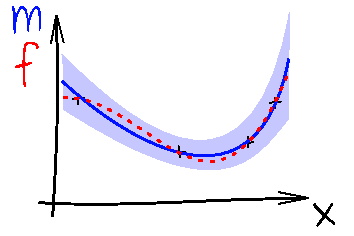
\includegraphics[height=5cm]{figures/ink_mconfint}
\end{center}
\end{frame}

%%%%%%%%%%%%%%%%%%%%%%%%%%%%%%%%%%%%%%%%%%%%%%%%%%%%%%
%%%%%%%%%%%%%%%%%%%%%%%%%%%%%%%%%%%%%%%%%%%%%%%%%%%%%%
\section{Linear Regression}
\subsection{}

%%%%%%%%%%%%%%%%%%%%%%%%%%%%%%%%%%%%%%%%%%%%%%%%%%%%%%
\begin{frame}{}
\begin{example}
	If we consider the following observations: 
\begin{center}
  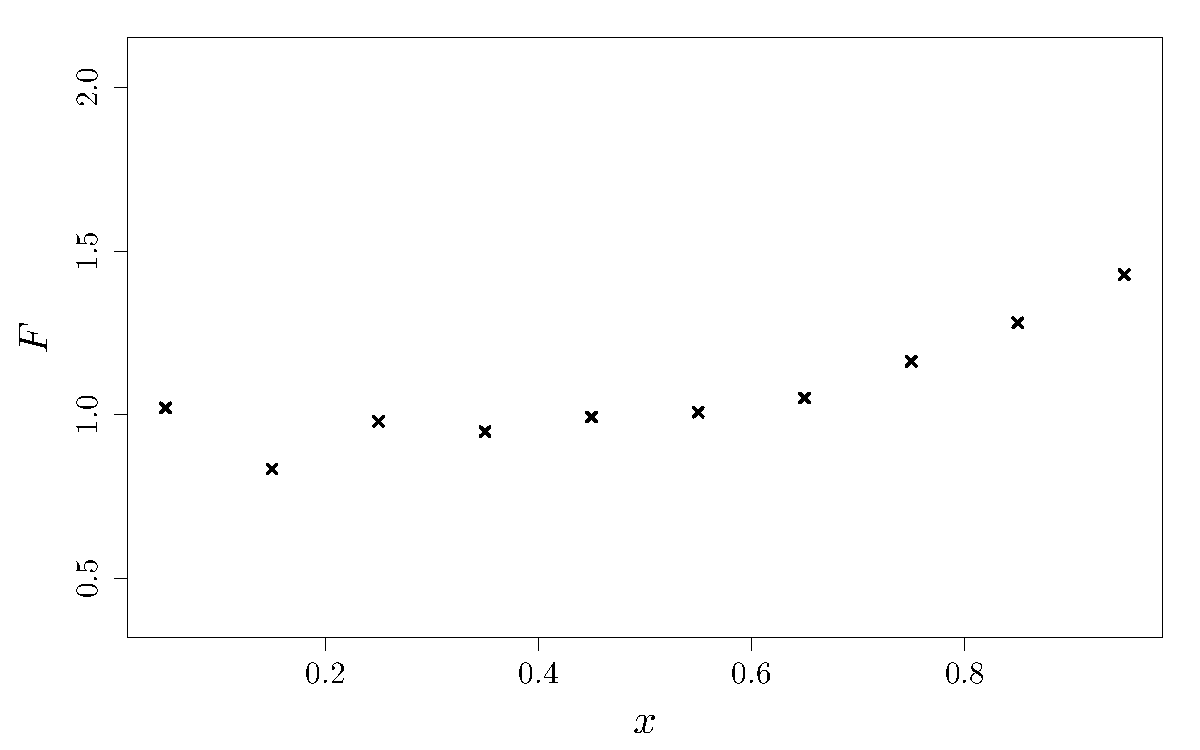
\includegraphics[height=5cm]{figures/R/linreg_0}
\end{center}
\vspace{-2mm}
\end{example}
\end{frame}

%%%%%%%%%%%%%%%%%%%%%%%%%%%%%%%%%%%%%%%%%%%%%%%%%%%%%%
\begin{frame}{}
\begin{example}
    We assume the observations are drawn from 
    $$ F_i = \sum_{k=0}^2 \beta_k b_k(X_i) + \varepsilon_i \qquad (= B(X_i) \beta  + \varepsilon_i )$$
	 with $b_0(x)=1,\ b_1(x)=x,\ b_2(x)=x^2$, unknown $\beta_i$ and i.i.d $\varepsilon_i$.
\begin{center}
  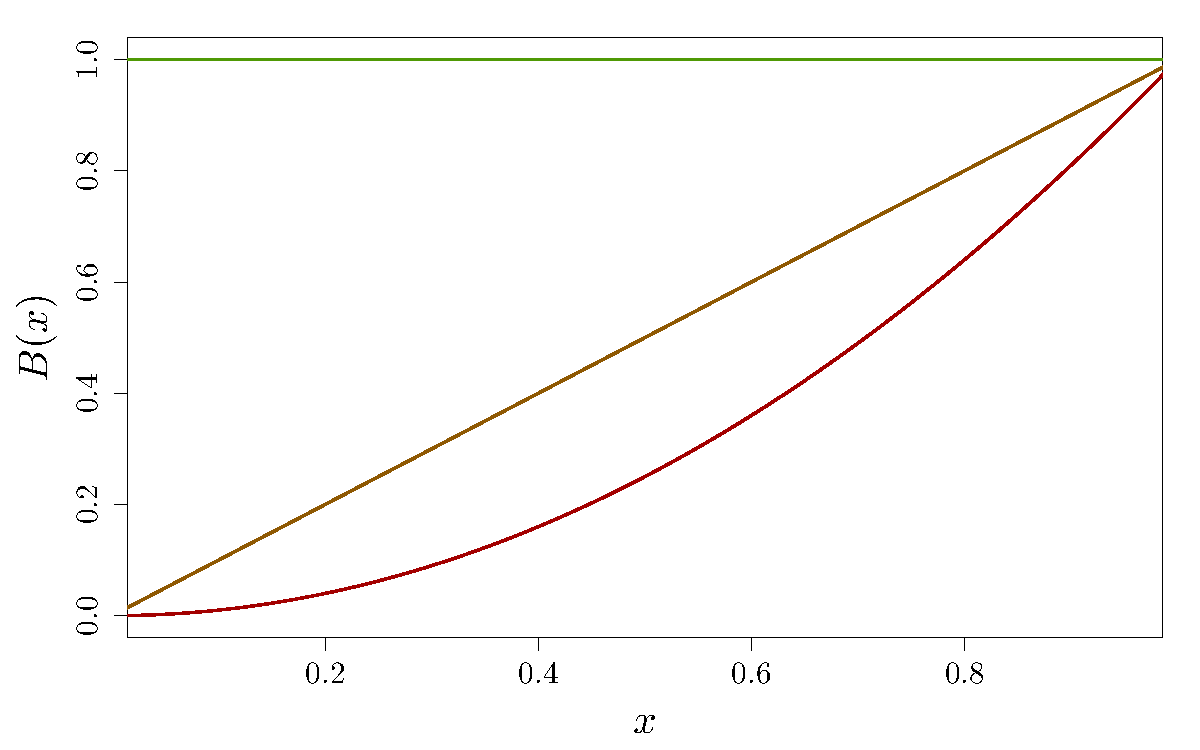
\includegraphics[height=4.9cm]{figures/R/linreg_1}
\end{center}
\end{example}
\end{frame}

%%%%%%%%%%%%%%%%%%%%%%%%%%%%%%%%%%%%%%%%%%%%%%%%%%%%%%
\begin{frame}{}
\begin{example}
The best linear unbiased estimator of $\beta$ is
$$\hat{\beta} = (B(X)^t B(X))^{-1} B(X)^t F.$$
We obtain $\hat{\beta} = (1.06,-0.61,1.04)^T$ and the model is:
\begin{center}
  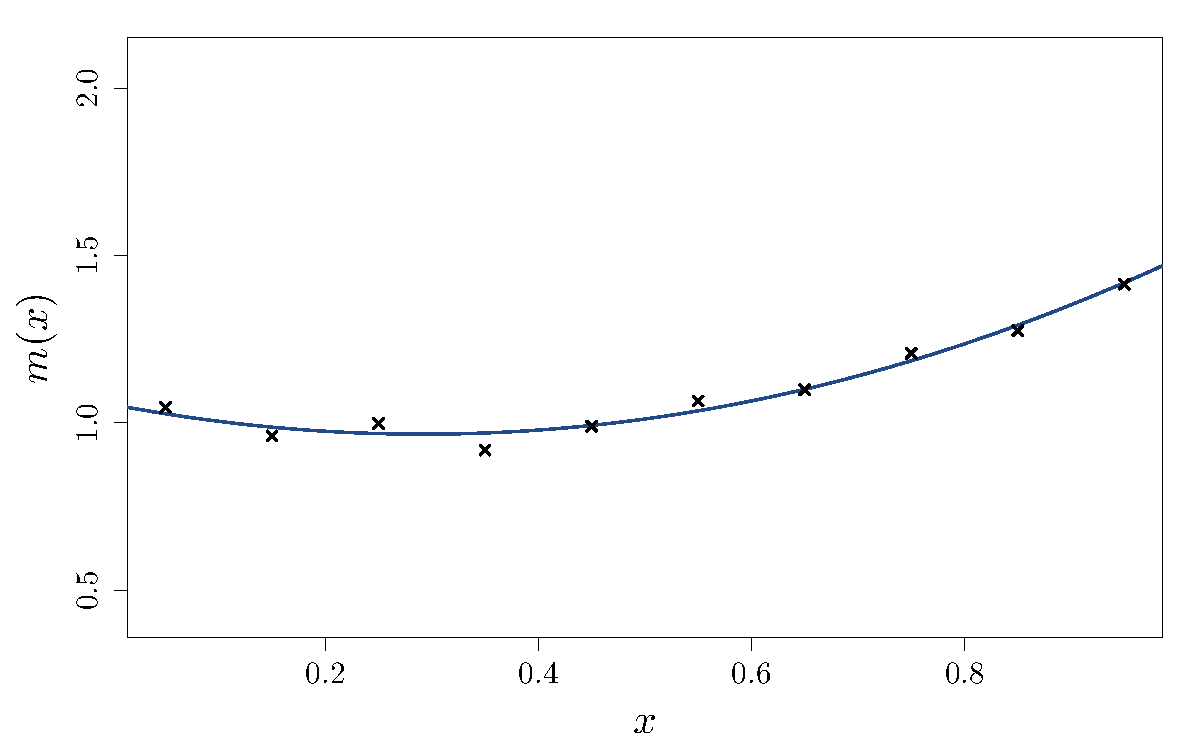
\includegraphics[height=5cm]{figures/R/linreg_2}
\end{center}
\end{example}
\end{frame}

%%%%%%%%%%%%%%%%%%%%%%%%%%%%%%%%%%%%%%%%%%%%%%%%%%%%%%
\begin{frame}{}
\begin{example}
There is of course an error between the true generative function and the model
\begin{center}
  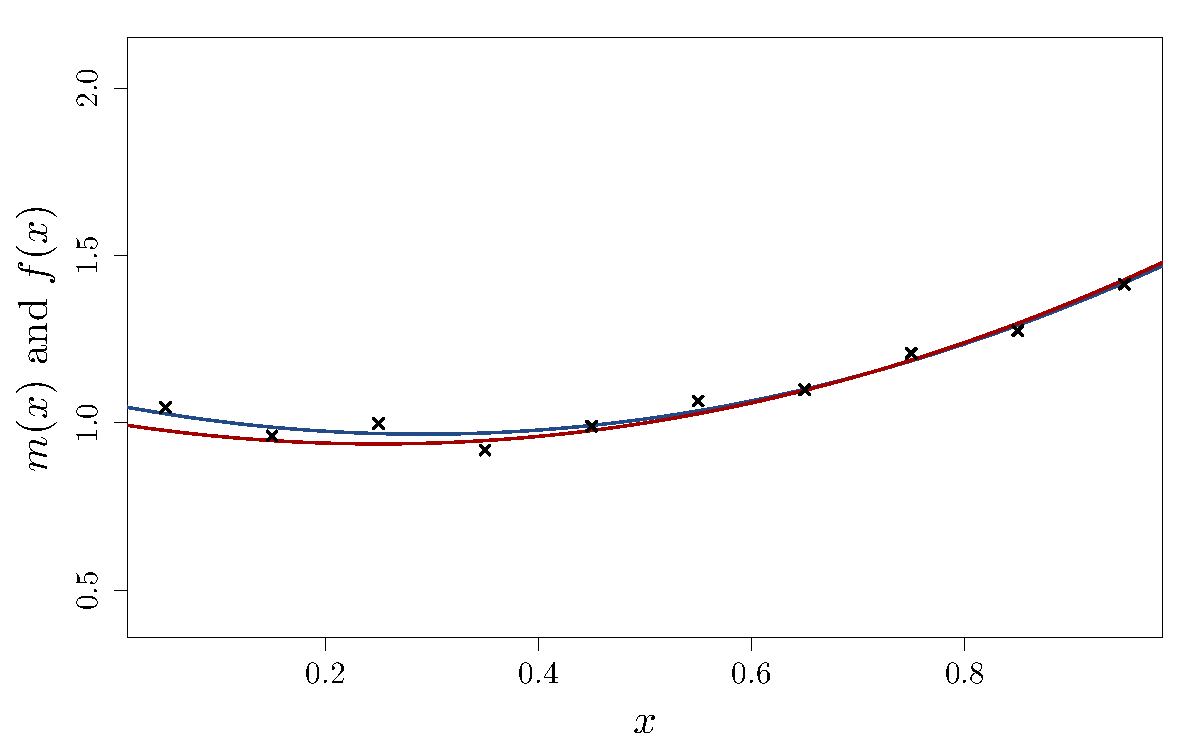
\includegraphics[height=5cm]{figures/R/linreg_3}
\end{center}
Can this error be quantified?
\end{example}
\end{frame}

%%%%%%%%%%%%%%%%%%%%%%%%%%%%%%%%%%%%%%%%%%%%%%%%%%%%%%
\begin{frame}{}
The estimator can also be seen as a random variable: 
$$\hat{\beta} = (B(X)^t B(X))^{-1} B(X)^t (B(X) \beta  + \varepsilon).$$ \\
\vspace{5mm}
\begin{itemize}
	\item Its expectation is $\beta$ \alert{$\Rightarrow$} The estimator is unbiased
	\item Its covariance matrix is $$(B(X)^t B(X))^{-1} B(X)^t \Cov[\varepsilon,\varepsilon^t] B(X) (B(X)^t B(X))^{-1}$$
	\item If $\varepsilon$ is multivariate normal, then $\hat{\beta}$ is also multivariate normal.
\end{itemize}
\end{frame}


% %%%%%%%%%%%%%%%%%%%%%%%%%%%%%%%%%%%%%%%%%%%%%%%%%%%%%%
% \begin{frame}{}
% The initial assumption is $ F = B(X) \beta  + \varepsilon$ and we have computed an estimator of $\beta$:
% $$\hat{\beta} = (B(X)^t B(X))^{-1} B(X)^t F.$$
% $\hat{\beta}$ can thus be seen as a sample from the random variable:
% $$\hat{\beta} = (B(X)^t B(X))^{-1} B(X)^t (B(X) \beta  + \varepsilon).$$ \\
% \vspace{5mm}
% What about the distribution of $\hat{\beta}$? \pause
% \begin{itemize}
% 	\item Its expectation is $\beta$ \alert{$\Rightarrow$} The estimator is unbiased
% 	\item Its covariance matrix is $$(B(X)^t B(X))^{-1} B(X)^t \Cov[\varepsilon,\varepsilon^t] B(X) (B(X)^t B(X))^{-1}$$
% 	\item If $\varepsilon$ is multivariate normal, then $\hat{\beta}$ is also multivariate normal.
% \end{itemize}
% \end{frame}
% 
% %%%%%%%%%%%%%%%%%%%%%%%%%%%%%%%%%%%%%%%%%%%%%%%%%%%%%%
% \begin{frame}{}
% Sampling in the distribution of $\hat{\beta}$ gives us a large variety of models which represent the uncertainty about our estimation:
% \begin{exampleblock}{Back to the example}
% \begin{center}
%   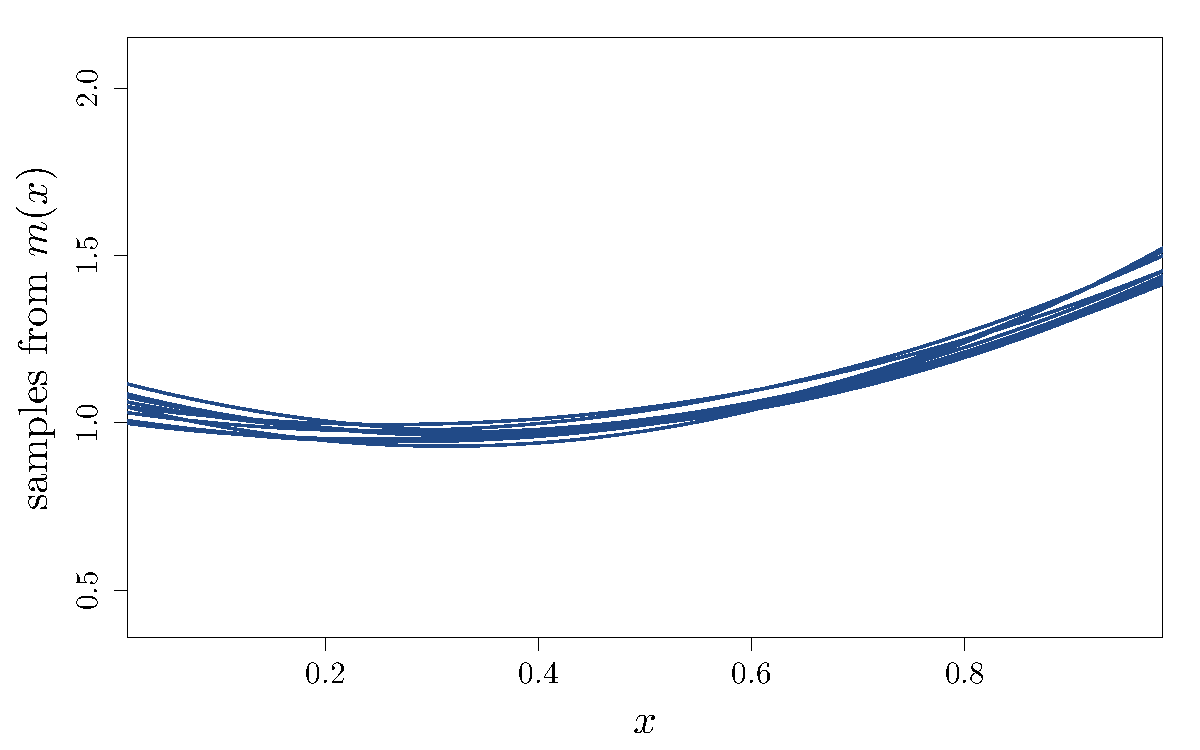
\includegraphics[height=5cm]{figures/R/linreg_4}
% \end{center}
% \end{exampleblock}
% \end{frame}

%%%%%%%%%%%%%%%%%%%%%%%%%%%%%%%%%%%%%%%%%%%%%%%%%%%%%%
\begin{frame}{}
\begin{exampleblock}{Back to the example}
Be obtain uncertainty on the model
\begin{center}
  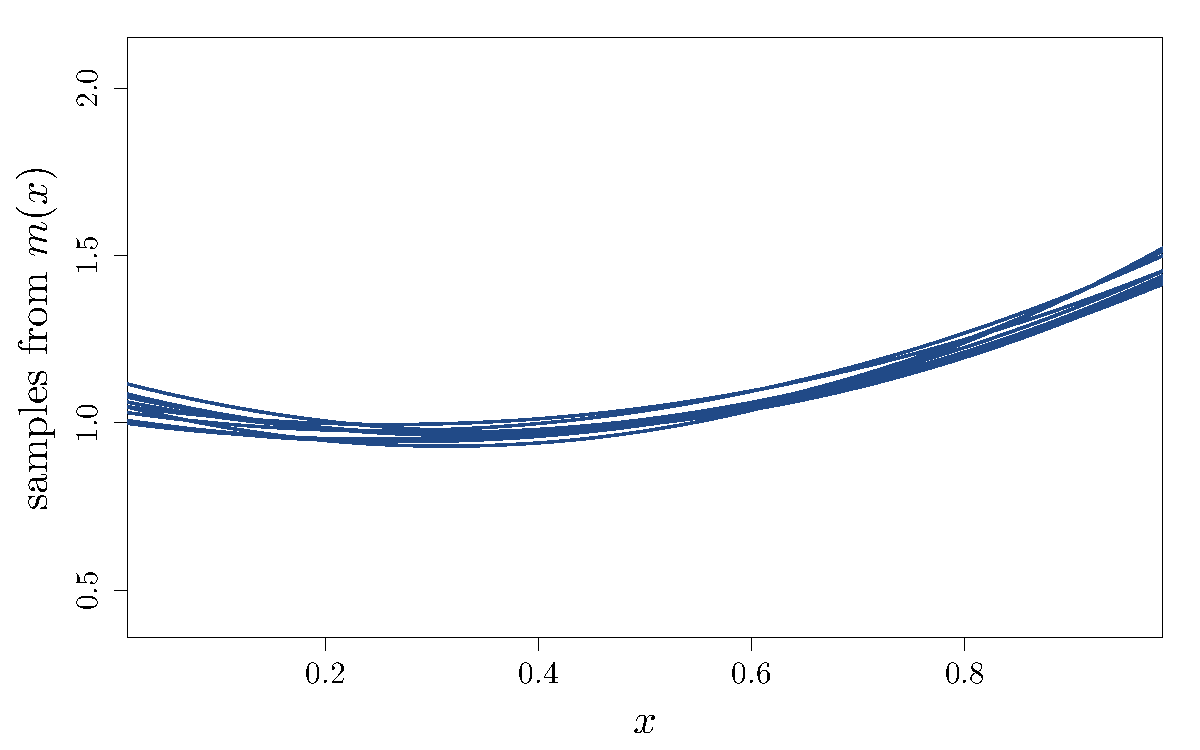
\includegraphics[height=5cm]{figures/R/linreg_4}
\end{center}
\end{exampleblock}
\end{frame}


%%%%%%%%%%%%%%%%%%%%%%%%%%%%%%%%%%%%%%%%%%%%%%%%%%%%%%
\begin{frame}{}
\begin{exampleblock}{Back to the example}
The previous picture can be summarized by showing the mean of $m$ and $95\%$ confidence intervals
\begin{center}
  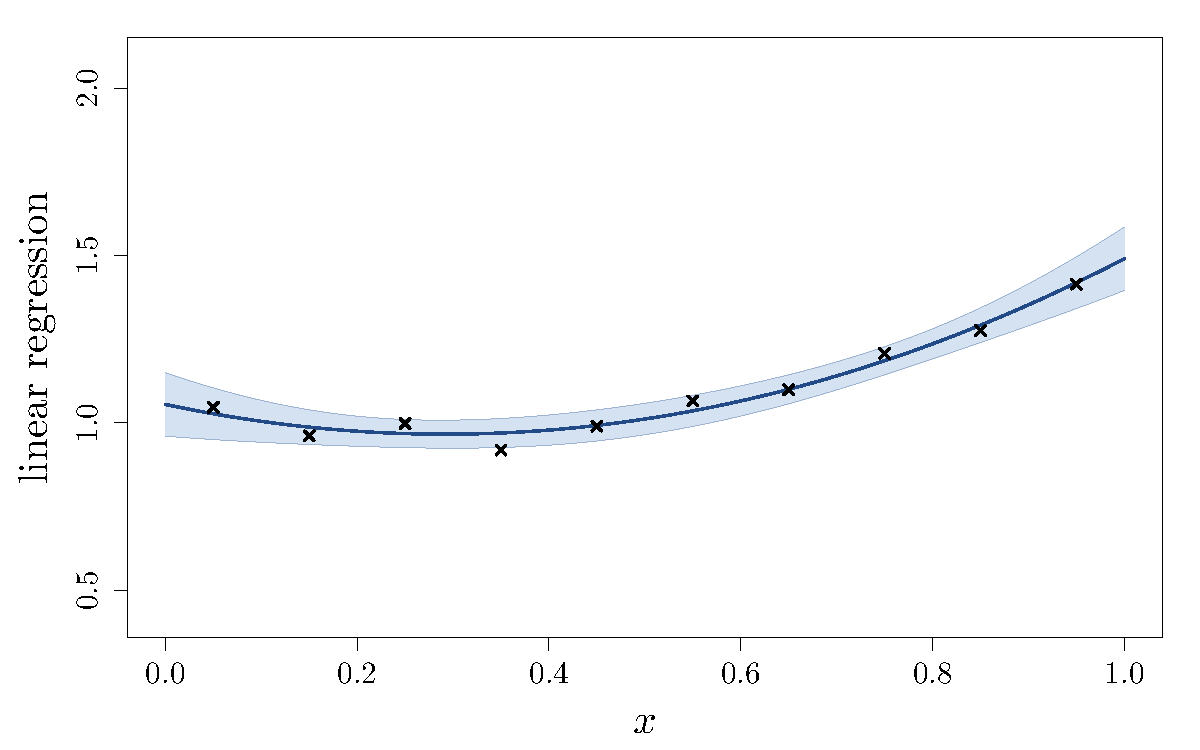
\includegraphics[height=5cm]{figures/R/linreg_5}
\end{center}
\end{exampleblock}
\end{frame}

%%%%%%%%%%%%%%%%%%%%%%%%%%%%%%%%%%%%%%%%%%%%%%%%%%%%%%
\begin{frame}{}
    This statistical model can be used for \textbf{uncertainty quantification}:
\begin{exampleblock}{Back to the example}
If we are interested in the value $x^\star$ minimizing $f(x)$:
\begin{center}
  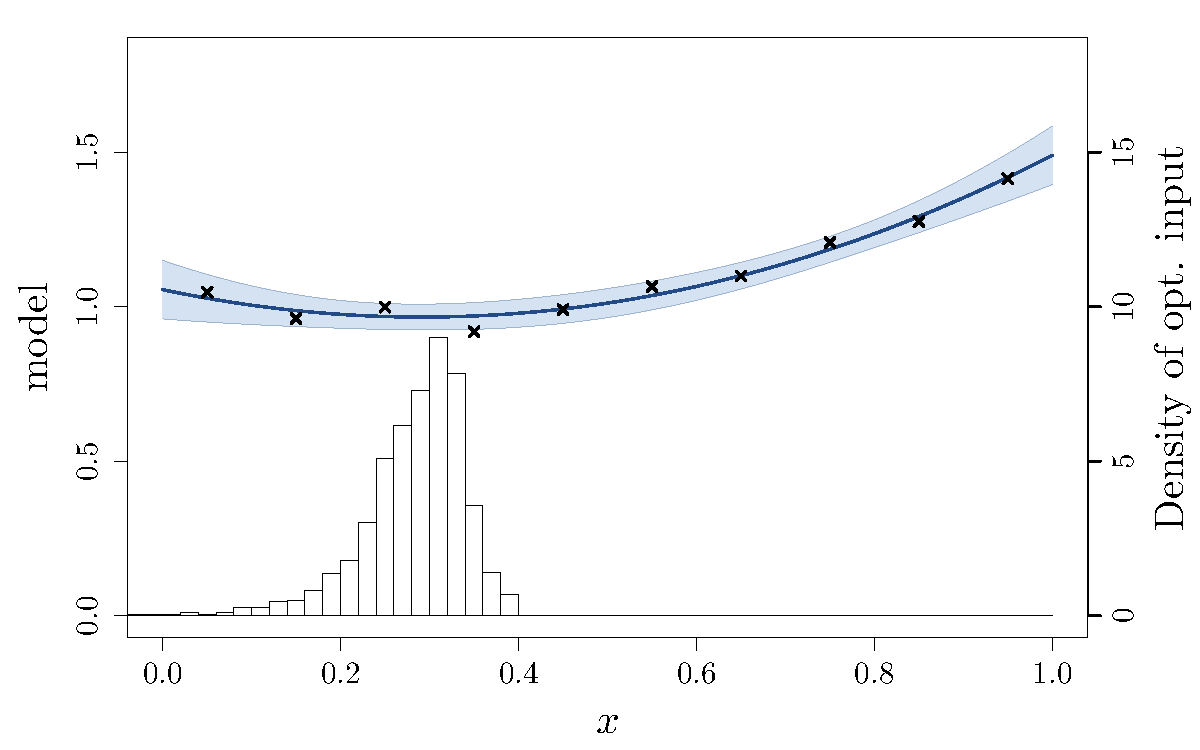
\includegraphics[height=5cm]{figures/R/linreg_6}
\end{center}
\end{exampleblock}
\alert{we obtain a distribution for $x^\star$.}
\end{frame}

%%%%%%%%%%%%%%%%%%%%%%%%%%%%%%%%%%%%%%%%%%%%%%%%%%%%%%
\begin{frame}{}
We could dedicate the entire course to linear regression models...
\begin{columns}[c]
\column{5cm}
\begin{itemize}
	\item model validation
	\item choice of basis functions
\end{itemize}
\column{6cm}
\begin{itemize}
	\item influence of input locations
	\item ...
\end{itemize}
\end{columns}
\vspace{10mm}
We will just stress a few \textbf{pros and cons of these models}:
\begin{itemize}
  \item[+] provide a good noise filtering
  \item[+] are easy to interpret
  \item[] \vspace{-5mm}
  \item[$-$] are not flexible (need to choose the basis functions)
  \item[$-$] do not interpolate
  \item[$-$] may explode when using high order polynomials (over-fitting)
\end{itemize}
\end{frame}

%%%%%%%%%%%%%%%%%%%%%%%%%%%%%%%%%%%%%%%%%%%%%%%%%%%%%%
%%%%%%%%%%%%%%%%%%%%%%%%%%%%%%%%%%%%%%%%%%%%%%%%%%%%%%
\section[Gaussian Process regression]{Gaussian Process Regression}
\subsection{}
%%%%%%%%%%%%%%%%%%%%%%%%%%%%%%%%%%%%%%%%%%%%%%%%%%%%%%
\begin{frame}{}
\vspace{0.75cm}
\structure{This section is organised in 3 subsections:}
\vspace{0.5cm}
\begin{enumerate}
    \item Univariate and multivariate normal distributions
    \item Gaussian processes
    \item Gaussian process regression
\end{enumerate}
\end{frame}

%%%%%%%%%%%%%%%%%%%%%%%%%%%%%%%%%%%%%%%%%%%%%%%%%%%%%%%%%%%%
%\subsection{Multivariate normal distribution}

%%%%%%%%%%%%%%%%%%%%%%%%%%%%%%%%%%%%%%%%%%%%%%%%%%%%%%
\begin{frame}{1D normal distribution}
We say that $X \sim \mathcal{N}(\mu,\sigma^2)$ if it has the following pdf:
\begin{columns}
  \begin{column}{0.6\textwidth}
  \begin{equation*}
  f(x) = \frac{1}{\sigma \sqrt{2 \pi}} \exp \left(-\frac{(x-\mu)^2}{2 \sigma^2} \right)
  \vspace{3mm}
  \end{equation*}
  The distribution is characterised by\\
      \qquad mean: $\mu = \E [X]$\\
      \qquad variance: $\sigma^2 = \E [X^2] - \E[X]^2$
  \end{column}
  \begin{column}{0.5\textwidth}
  \begin{center}
   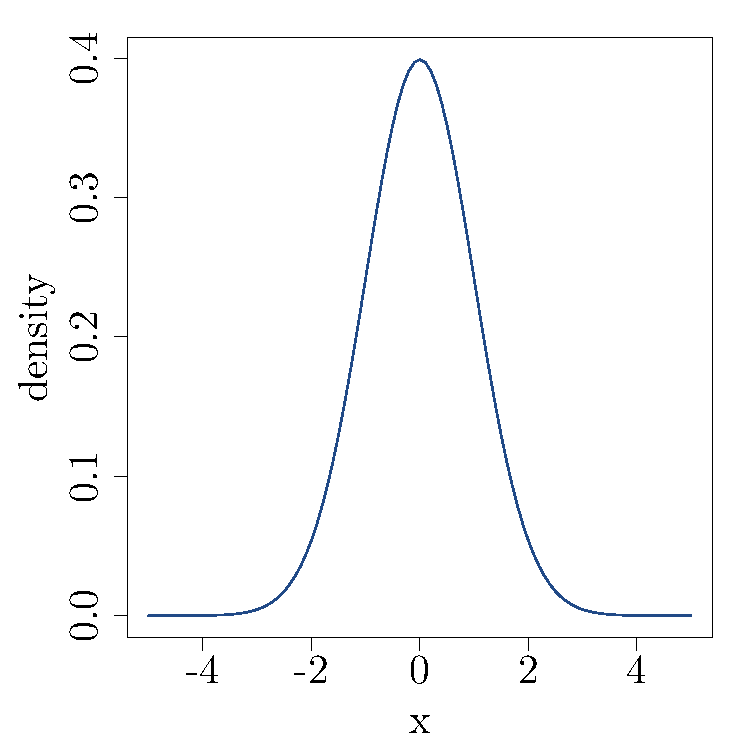
\includegraphics[height=4.7cm]{figures/R/MVN_dens1} 
  \end{center}
  \end{column}
\end{columns}
\vspace{2mm}
\structure{One fundamental property:} a linear combination of independant normal distributed random variables is still normal distributed.
\end{frame}

%%%%%%%%%%%%%%%%%%%%%%%%%%%%%%%%%%%%%%%%%%%%%%%%%%%%%%
\begin{frame}{Multivariate normal distribution}
\begin{definition}
	We say that a vector $Y=(Y_1, \dots, Y_n)^t$ follows a multivariate normal distribution if any linear combination of $Y$ follows a normal distribution:
	\begin{equation*}
		\forall \alpha \in \mathds{R}^n,\ \alpha^t Y \sim \mathcal{N}
	\end{equation*}
\end{definition}
The distribution of a Gaussian vector is characterised by
\begin{itemize}
 	\item a \textbf{mean vector} $\mu = \E [Y]$
 	\item a \textbf{covariance matrix} $\Sigma = \E[YY^t] - \E[Y] \E[Y]^t$ % \hfill (i.e. $\Sigma_{i,j}=\Cov(Y_i, Y_j)$)
\end{itemize}
\vspace{3mm}
\structure{Property:}\\
A covariance matrix is
\begin{itemize}
	\item symmetric $K_{i,j}=K_{j,i}$
	\item positive semi-definite $\forall \alpha \in \mathds{R}^n, \alpha^t K \alpha \geq 0$.
\end{itemize}
\end{frame}

%%%%%%%%%%%%%%%%%%%%%%%%%%%%%%%%%%%%%%%%%%%%%%%%%%%%%%
\begin{frame}{}
The pdf of a multivariate Gaussian is:
\begin{equation*}
f_Y(x) = \frac{1}{\displaystyle (2 \pi)^{n/2} |\Sigma|^{1/2}} \exp \left(-\frac12 (x-\mu)^t K^{-1} (x-\mu)  \right).
\end{equation*}
\begin{center}
 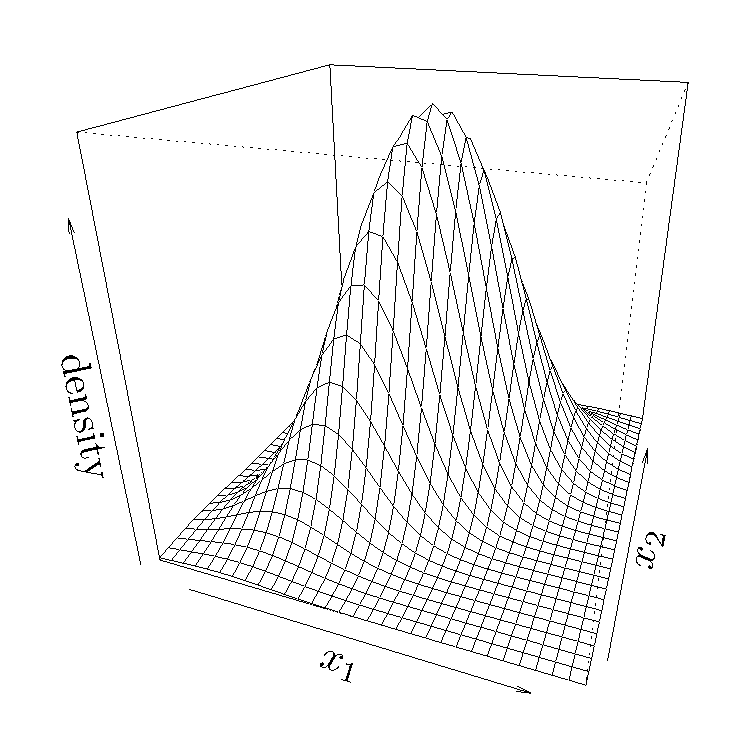
\includegraphics[height=5cm]{figures/R/MVN_dens2}
\end{center}
\end{frame}


%%%%%%%%%%%%%%%%%%%%%%%%%%%%%%%%%%%%%%%%%%%%%%%%%%%%%%
\begin{frame}{}
\begin{exampleblock}{Samples from a multivariate normal}
 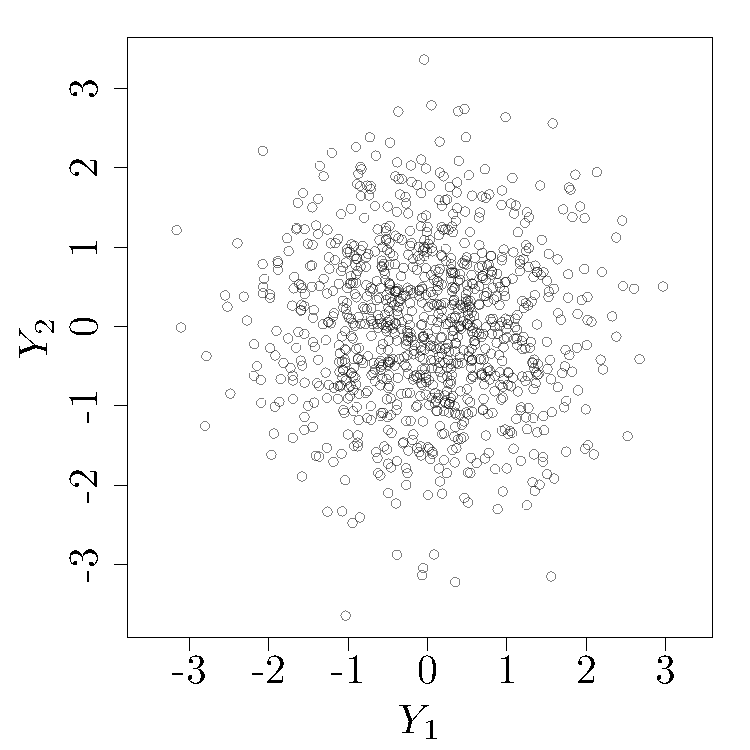
\includegraphics[height=4.5cm]{figures/R/MVN_gaussvec2} \qquad \qquad 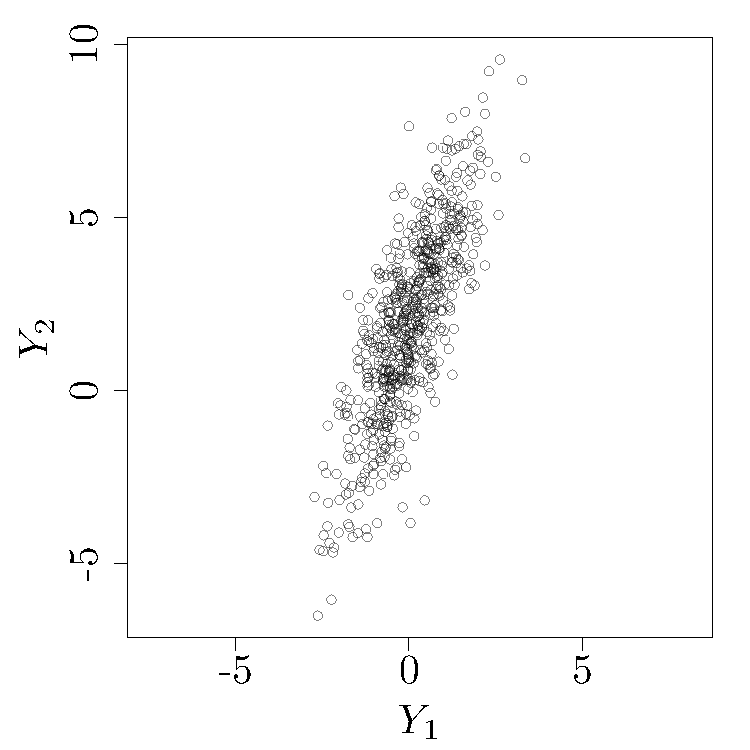
\includegraphics[height=4.5cm]{figures/R/MVN_gaussvec1}
\end{exampleblock}
\vspace{-5mm}
\begin{exampleblock}{Exercise}
\begin{itemize}
  \item For $X=(X_1,\dots,X_n)$ with $X_i$ independent and $\mathcal{N}(0,1)$, and a $n \times n$ matrix $A$, what is the distribution of $AX$?
  \item For a given covariance matrix $K$ and independent $\mathcal{N}(0,1)$ samples, how can we generate $\mathcal{N}(\mu,K)$ random samples?
\end{itemize}
\end{exampleblock}
% \alert{$\Rightarrow$ R demo}
\end{frame}

%%%%%%%%%%%%%%%%%%%%%%%%%%%%%%%%%%%%%%%%%%%%%%%%%%%%%%
\begin{frame}{}
\begin{exampleblock}{Counter example}
\begin{center}
 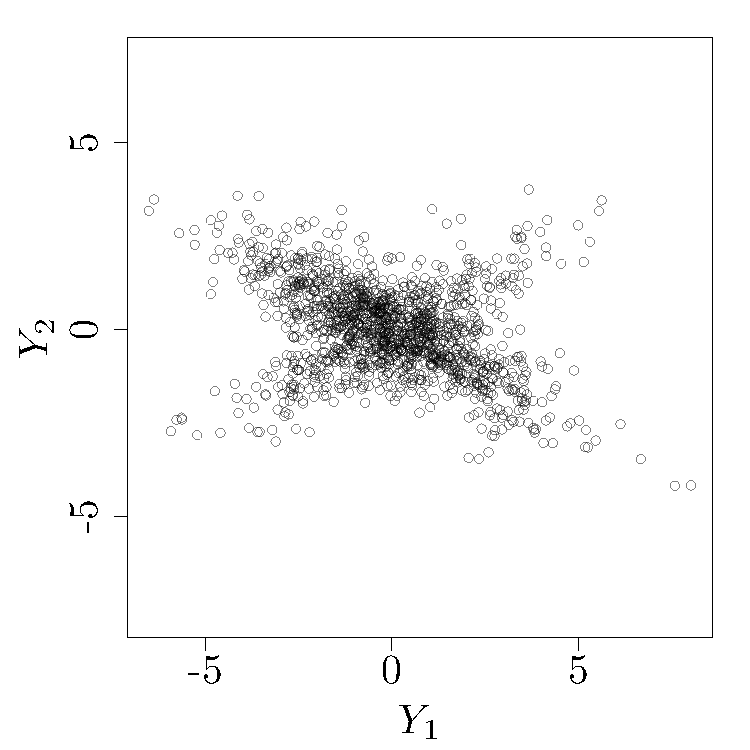
\includegraphics[height=5cm]{figures/R/MVN_gaussvec3}
\end{center}
$Y_1$ and $Y_2$ are normally distributed but \textbf{the couple $(Y_1,Y_2)$ is not}.
\end{exampleblock}
\end{frame}

%%%%%%%%%%%%%%%%%%%%%%%%%%%%%%%%%%%%%%%%%%%%%%%%%%%%%%
\begin{frame}{}
\begin{block}{Conditional distribution}
2D multivariate Gaussian conditional distribution:\\
\begin{columns}
\begin{column}{5cm}
\begin{align*}
p(y_1 | y_2=\alpha) & = \frac{p(y_1,\alpha)}{p(\alpha)}\\[2mm]
& = \frac{\exp({\color{myDarkPurple} \mathrm{quadratic\ in\ } y_1 \mathrm{\ and\ } \alpha})}{\mathrm{const}}\\[2mm]
& = \frac{\exp({\color{myDarkPurple} \mathrm{quadratic\ in\ } y_1})}{\mathrm{const}}\\[2mm]
%& = \exp({\color{myDarkPurple} \mathrm{quadratic\ in\ } y_1})\\[2mm]
& = \mathrm{Gaussian\ distribution!}
\end{align*}
\end{column}
\begin{column}{5cm}
\begin{center}
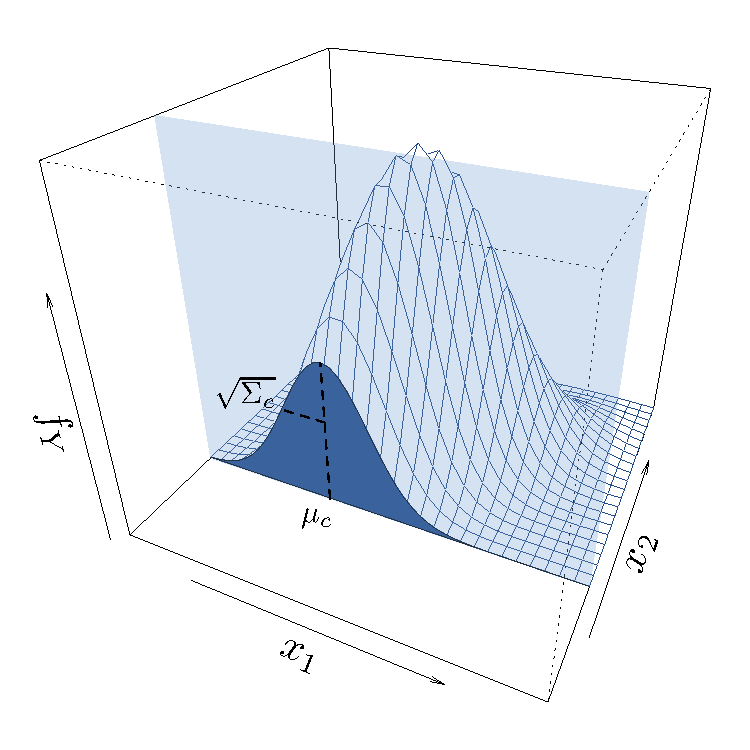
\includegraphics[height=5cm]{figures/ch1_condpdf1}
\end{center}
\end{column}
\end{columns}
The conditional distribution is still Gaussian!
\end{block}
\end{frame}

%%%%%%%%%%%%%%%%%%%%%%%%%%%%%%%%%%%%%%%%%%%%%%%%%%%%%%
\begin{frame}{}
\begin{block}{Conditional distribution}
Let $(Y_1,Y_2)$ be a Gaussian vector ($Y_1$ and $Y_2$ may both be vectors):
\begin{equation*}
\begin{pmatrix}
	Y_1\\
	Y_2\\
\end{pmatrix}
=
\mathcal{N}
\left(
\begin{pmatrix}
	\mu_1\\
	\mu_2\\
\end{pmatrix},
\begin{pmatrix}
	\Sigma_{11} & \Sigma_{12}\\
	\Sigma_{21} & \Sigma_{22}\\
\end{pmatrix}
\right).
\vspace{5mm}
\end{equation*}
The conditional distribution of $Y_1$ given $Y_2$ is:
 $$Y_1|Y_2 \sim \mathcal{N}(\mu_\mathrm{cond},\Sigma_\mathrm{cond})$$
\begin{equation*}
\begin{split}
	\text{with \qquad} \mu_\mathrm{cond} &= \E [Y_1|Y_2] = \mu_1 + \Sigma_{12} \Sigma_{22}^{-1} (Y_2-\mu_2)\\
	\Sigma_\mathrm{cond} &= \Cov [Y_1,Y_1|Y_2] = \Sigma_{11} - \Sigma_{12} \Sigma_{22}^{-1} \Sigma_{21}
\end{split}
\end{equation*}
\end{block}
\end{frame}

%%%%%%%%%%%%%%%%%%%%%%%%%%%%%%%%%%%%%%%%%%%%%%%%%%%%%%
\begin{frame}{}
\begin{exampleblock}{3D Example}
3D multivariate Gaussian conditional distribution:\\
\begin{center}
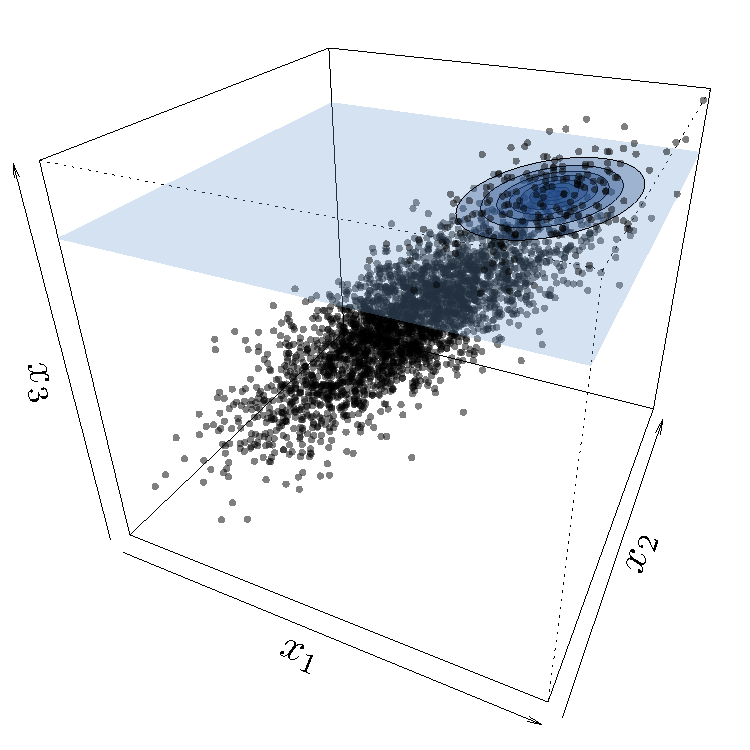
\includegraphics[height=6cm]{figures/ch1_condpdf2}
\end{center}
\end{exampleblock}
\end{frame}

%%%%%%%%%%%%%%%%%%%%%%%%%%%%%%%%%%%%%%%%%%%%%%%%%%%%%%
\begin{frame}{2. Gaussian processes}
The multivariate Gaussian distribution can be generalised to random processes:
\begin{definition}
A random process $Z$ over $D \subset \mathds{R}^d$ is said to be Gaussian if
\begin{equation*}
\forall n \in \mathds{N}, \forall x_i \in D, (Z(x_1),\dots,Z(x_n)) \text{  is a Gaussian vector}.
\end{equation*}
\end{definition}
The distribution of a GP is fully characterised by:
\begin{itemize}
	\item its mean function $m$ defined over $D$
	\item its covariance function (or kernel) $k$ defined over $D \times D$: $k(x,y) = \Cov(Z(x),Z(y))$
\end{itemize}
We will use the notation $Z \sim \mathcal{N}(m(.),k(.,.))$.\\
\end{frame}

%%%%%%%%%%%%%%%%%%%%%%%%%%%%%%%%%%%%%%%%%%%%%%%%%%%%%%
\begin{frame}{}
Let's look at the sample paths of a Gaussian Process!\\
\vspace{2mm}
\begin{center}
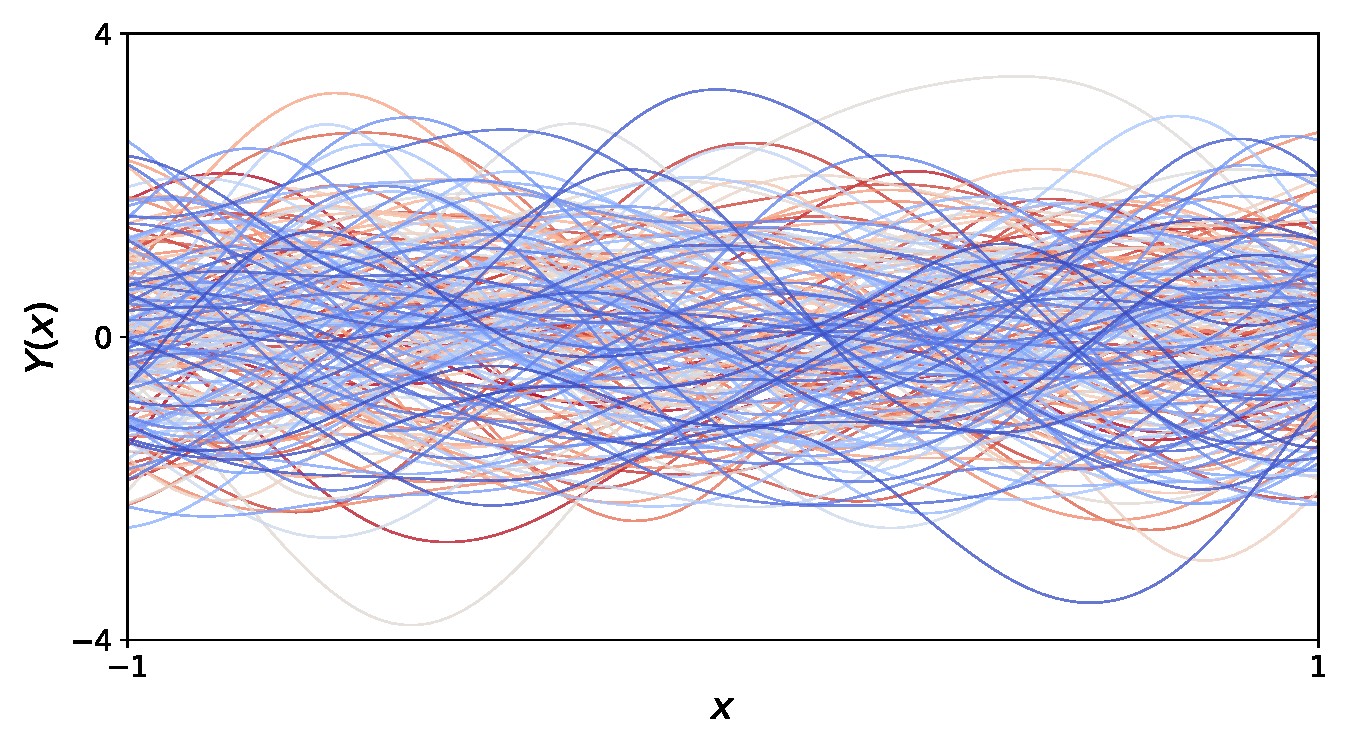
\includegraphics[height=5cm]{figures/python/gp_samples}
\end{center}
\end{frame}

%%%%%%%%%%%%%%%%%%%%%%%%%%%%%%%%%%%%%%%%%%%%%%%%%%%%%%
\begin{frame}{}
\begin{exampleblock}{Exercise: Simulating sample paths}
Let X be a set 100 regularly spaced points over the input space of $Z$.
\begin{itemize}
	\item What is the distribution of $Z(X)$ ?
	\item How to simulate samples from $Z(X)$ ?
\end{itemize}
\end{exampleblock}
\end{frame}

%%%%%%%%%%%%%%%%%%%%%%%%%%%%%%%%%%%%%%%%%%%%%%%%%%%%%%
\begin{frame}{}
A kernel satisfies the following properties:
\begin{itemize}
	\item It is symmetric: $k(x,y) = k(y,x)$
	\item It is positive semi-definite (psd):
\end{itemize}
\begin{equation*}
	\forall n \in \mathds{N}, \forall x_i \in D, \forall \alpha \in \mathds{R}^n,\  \sum_{i=1}^n \sum_{j=1}^n \alpha_i \alpha_j k(x_i,x_j) \geq 0
\end{equation*}
\vspace{5mm} \\
Furthermore any symmetric psd function can be seen as the covariance of a Gaussian process. This equivalence is known as the Loeve theorem.
\end{frame}

%%%%%%%%%%%%%%%%%%%%%%%%%%%%%%%%%%%%%%%%%%%%%%%%%%%%%%
\begin{frame}{}
There are a lot of functions that have already been proven psd:\\
\vspace{2mm}
\footnotesize
\begin{tabular}{rlN}
		constant & $ \displaystyle k(x,y) = \sigma^2 $ &\\[4mm]
		white noise & $ \displaystyle k(x,y) = \sigma^2 \delta_{x,y} $ &\\[4mm]
		Brownian & $ \displaystyle k(x,y) =  \sigma^2  \min (x,y) $ &\\[4mm]
		exponential & $\displaystyle k(x,y) =  \sigma^2 \exp \left(- |x-y|/\theta \right)$ &\\[4mm]
		Matern 3/2 & $\displaystyle k(x,y) =  \sigma^2 \left(1 + |x-y| \right) \exp \left(- |x-y| /\theta\right)$ &\\[4mm]
		Matern 5/2 & $\displaystyle k(x,y) =  \sigma^2 \left(1 + |x-y| /\theta+ 1/3|x-y|^2 /\theta^2 \right) \exp \left(- |x-y| /\theta\right)$ &\\[4mm]
		\hspace{-5mm}squared exponential & $\displaystyle k(x,y) =  \sigma^2 \exp \left(- (x-y)^2 /\theta^2 \right)$ &\\[4mm]
		$\vdots$ &
		% linear & $ \displaystyle k(x,y) = \sigma^2 xy $ &\\[4mm]
		% cosine & $ \displaystyle k(x,y) = \sigma^2 \cos \left (\frac{x-y}{\theta} \right) $ &\\[4mm]
		% sinc & $ \displaystyle k(x,y) = \sigma^2 \frac{\theta}{x-y} \sin \left( \frac{x-y}{\theta} \right) $ &\\[4mm] \hline
\end{tabular}\\
%%\begin{tabular}{rlN}
%%		constant & $ \displaystyle k(x,y) = 1 $ &\\[4mm]
%%		white noise & $ \displaystyle k(x,y) = \delta_{x,y} $ &\\[4mm]
%%		Brownian & $ \displaystyle k(x,y) =  \min (x,y) $ &\\[4mm]
%%		exponential & $\displaystyle k(x,y) = \exp \left(- |x-y| \right)$ &\\[4mm]
%%		Matern 3/2 & $\displaystyle k(x,y) = \left(1 + |x-y| \right) \exp \left(- |x-y| \right)$ &\\[4mm]
%%		Matern 5/2 & $\displaystyle k(x,y) = \left(1 + |x-y| + 1/3|x-y|^2 \right) \exp \left(- |x-y| \right)$ &\\[4mm]
%%		squared exponential & $\displaystyle k(x,y) = \exp \left(- (x-y)^2 \right)$ &\\[4mm]
%%		$\vdots$ &
%%		% linear & $ \displaystyle k(x,y) = \sigma^2 xy $ &\\[4mm]
%%		% cosine & $ \displaystyle k(x,y) = \sigma^2 \cos \left (\frac{x-y}{\theta} \right) $ &\\[4mm]
%%		% sinc & $ \displaystyle k(x,y) = \sigma^2 \frac{\theta}{x-y} \sin \left( \frac{x-y}{\theta} \right) $ &\\[4mm] \hline
%%\end{tabular}\\
\vspace{2mm}
\normalsize
The parameter $\sigma^2$ is called the \textbf{variance} and $\theta$ the \textbf{length-scale}.\\
\alert{$\Rightarrow$ Shiny App:} \url{https://github.com/NicolasDurrande/shinyApps} \\
\end{frame}

%% %%%%%%%%%%%%%%%%%%%%%%%%%%%%%%%%%%%%%%%%%%%%%%%%%%%%%%
%% \begin{frame}{}
%% In higher dimension one can introduce one length-scale parameter per dimension. The usual Euclidean distance between two points $|| x-y || = ( \sum (x_i-y_i)^2)^{1/2}$ is thus replaced by
%% \begin{equation*}
%% 	\Ni{x-y}{\theta} = \left( \sum_{i=1}^d \frac{(x_i-y_i)^2}{\theta_i^2} \right)^{1/2}.
%% \end{equation*}
%% If the parameters $\theta_i$ are equal for all the dimensions, the covariance (or the process) is called \textbf{isotropic}.\\
%% \vspace{5mm}
%% \alert{$\Rightarrow$ R demo}
%% \end{frame}

%%%%%%%%%%%%%%%%%%%%%%%%%%%%%%%%%%%%%%%%%%%%%%%%%%%%%%
\begin{frame}{}
Here is a list of the most common kernels in higher dimension:\\
\vspace{2mm}
\footnotesize
% \centering
\begin{tabular}{rlN}
		constant & $ \displaystyle k(x,y) = \sigma^2 $ &\\[4mm]
		white noise & $ \displaystyle k(x,y) = \sigma^2 \delta_{x,y} $ &\\[4mm]
		exponential & $\displaystyle k(x,y) = \sigma^2 \exp \left(- \Ni{x-y}{\theta} \right)$ &\\[4mm]
		Matern 3/2 & $\displaystyle k(x,y) = \sigma^2 \left(1 + \sqrt{3}\Ni{x-y}{\theta} \right) \exp \left(- \sqrt{3}\Ni{x-y}{\theta}  \right)$ &\\[4mm]
		Matern 5/2 & $\displaystyle k(x,y) = \sigma^2 \left(1 + \sqrt{5}\Ni{x-y}{\theta} + \frac{5}{3}\Ni{x-y}{\theta}^2 \right) \exp \left(- \sqrt{5}\Ni{x-y}{\theta} \right)$ &\\[4mm]
		Gaussian & $\displaystyle k(x,y) = \sigma^2 \exp \left(- \frac12 \Ni{x-y}{\theta}^2 \right)$ &\\[4mm]
\end{tabular}
\normalsize where
\begin{equation*}
	\Ni{x-y}{\theta} = \left( \sum_{i=1}^d \frac{(x_i-y_i)^2}{\theta_i^2} \right)^{1/2}.
\end{equation*}
\alert{$\Rightarrow$ R demo}
\end{frame}

%%%%%%%%%%%%%%%%%%%%%%%%%%%%%%%%%%%%%%%%%%%%%%%%%%%%%%%%%%%%
%\subsection{Gaussian process regression}

%%%%%%%%%%%%%%%%%%%%%%%%%%%%%%%%%%%%%%%%%%%%%%%%%%%%%%
\begin{frame}{ Gaussian process regression}
We assume we have observed a function $f$ for a set of points $X = (X_1,\dots,X_n)$:
\begin{center}
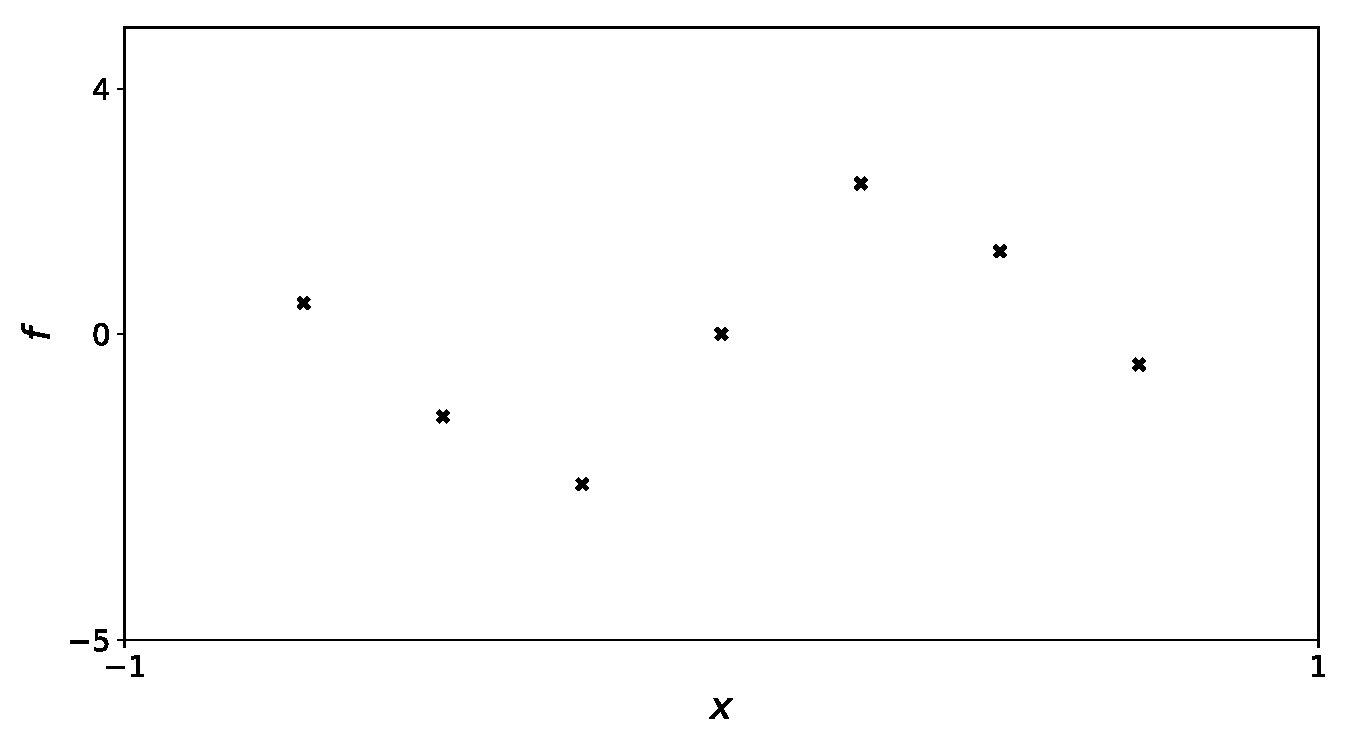
\includegraphics[height=5cm]{figures/python/gp_obs}
\end{center}
The vector of observations is $F=f(X)$ (ie $F_i = f(X_i)$ ).
\end{frame}

%%%%%%%%%%%%%%%%%%%%%%%%%%%%%%%%%%%%%%%%%%%%%%%%%%%%%%
\begin{frame}{}
Since $f$ in unknown, we make the general assumption that
it is the sample path of a Gaussian process $Z \sim \mathcal{N}(0,k)$:
\begin{center}
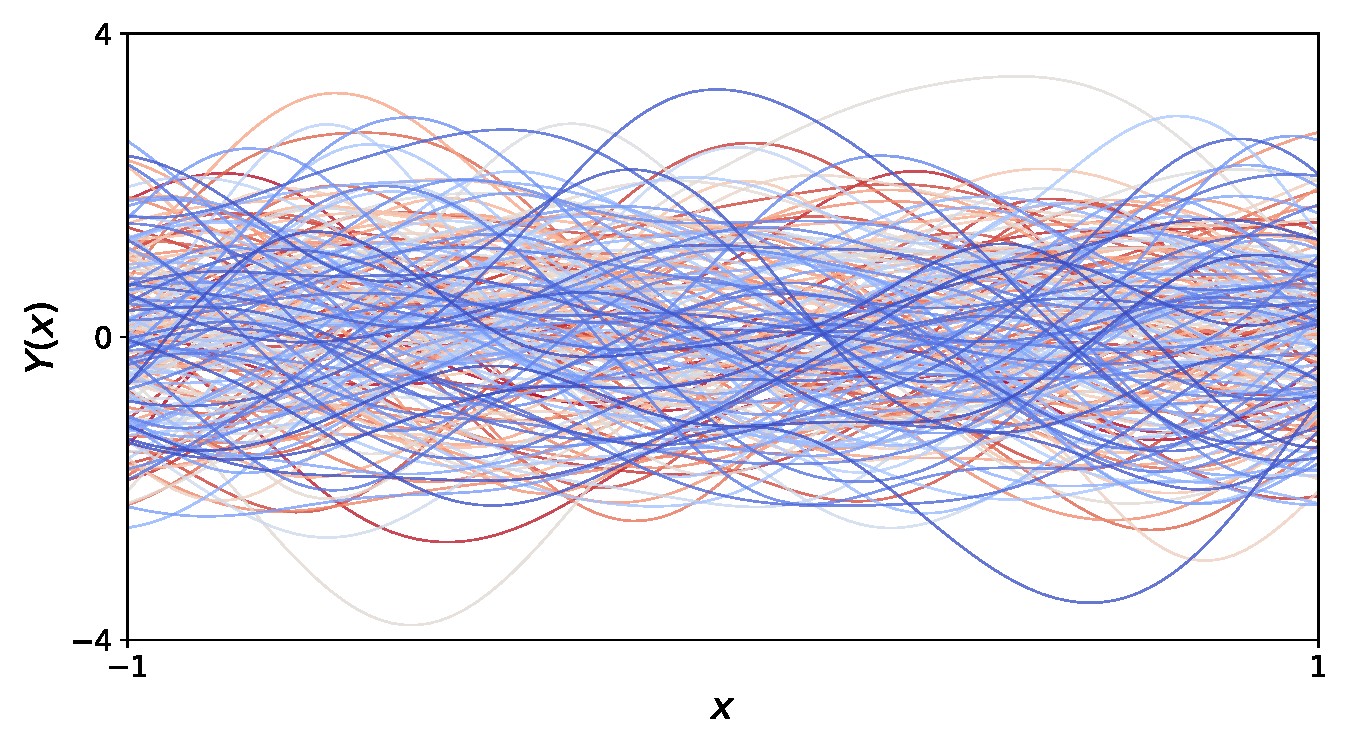
\includegraphics[height=5cm]{figures/python/gp_samples}
\end{center}
\end{frame}

%%%%%%%%%%%%%%%%%%%%%%%%%%%%%%%%%%%%%%%%%%%%%%%%%%%%%%
\begin{frame}{}
    \vspace{5mm}
    The posterior distribution $\gp(\cdot)|\gp(X)=\obs$: \\
    \begin{itemize}
        \item Is still Gaussian
        \item Can be computed analytically
    \end{itemize}
    \vspace{3mm}
    It is $\mathcal{N}(m(\cdot),c(\cdot,\cdot))$ with:
    \begin{equation*}
        \begin{split}
            m(x) &= \E[\gp(x)|\gp(X) \shorteq \obs] \\
            &= k(x,X) k(X,X)^{-1} \obs \\[3mm]
            c(x,y) &= \Cov[\gp(x),\gp(y)|\gp(X) \shorteq \obs] \\
            &= k(x,y) - k(x,X) k(X,X)^{-1} k(X,y)
        \end{split}
    \end{equation*}
\end{frame}


%%%%%%%%%%%%%%%%%%%%%%%%%%%%%%%%%%%%%%%%%%%%%%%%%%%%%%
\begin{frame}{}
    \vspace{5mm}
    Samples from the posterior distribution\\
    \centering
    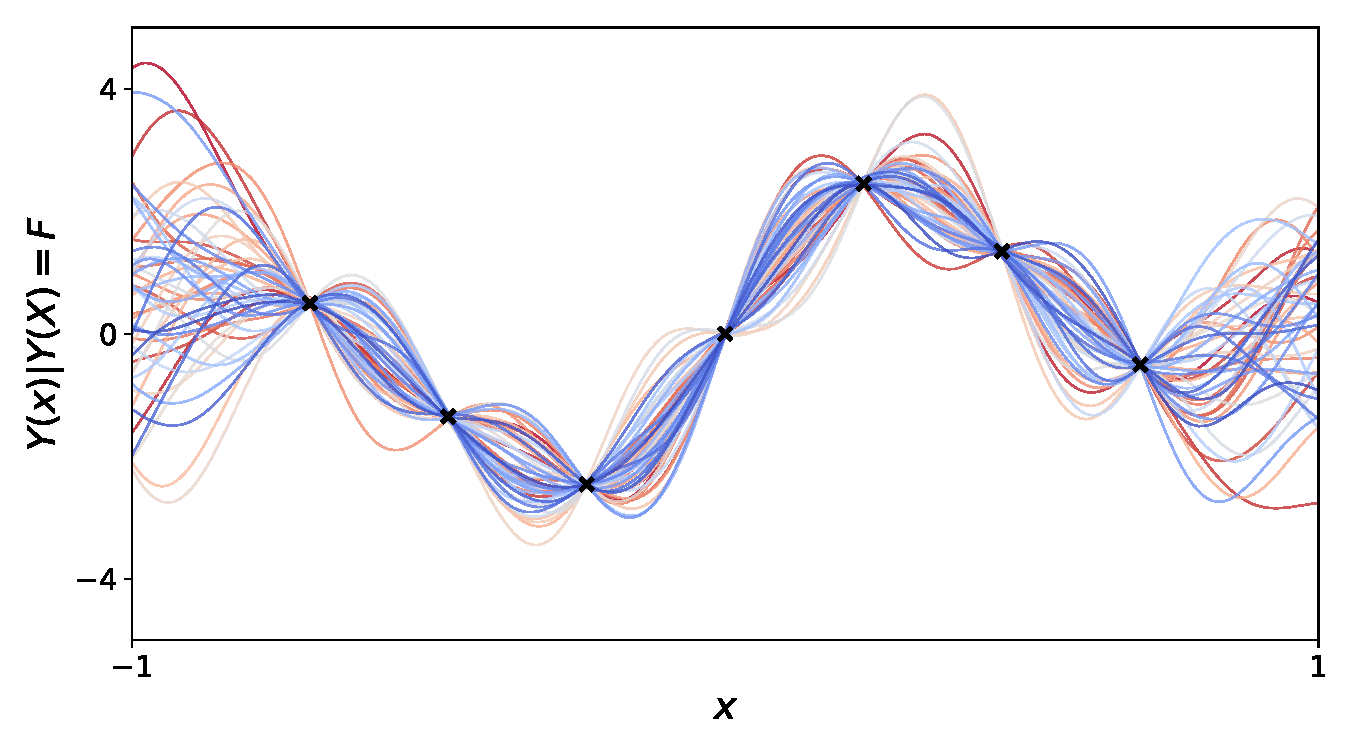
\includegraphics[height=6cm]{figures/python/gp_cond_samples}
\end{frame}

%%%%%%%%%%%%%%%%%%%%%%%%%%%%%%%%%%%%%%%%%%%%%%%%%%%%%%
\begin{frame}{}
    \vspace{5mm}
    It can be summarized by a mean function and 95\% confidence intervals.\\
    \centering
    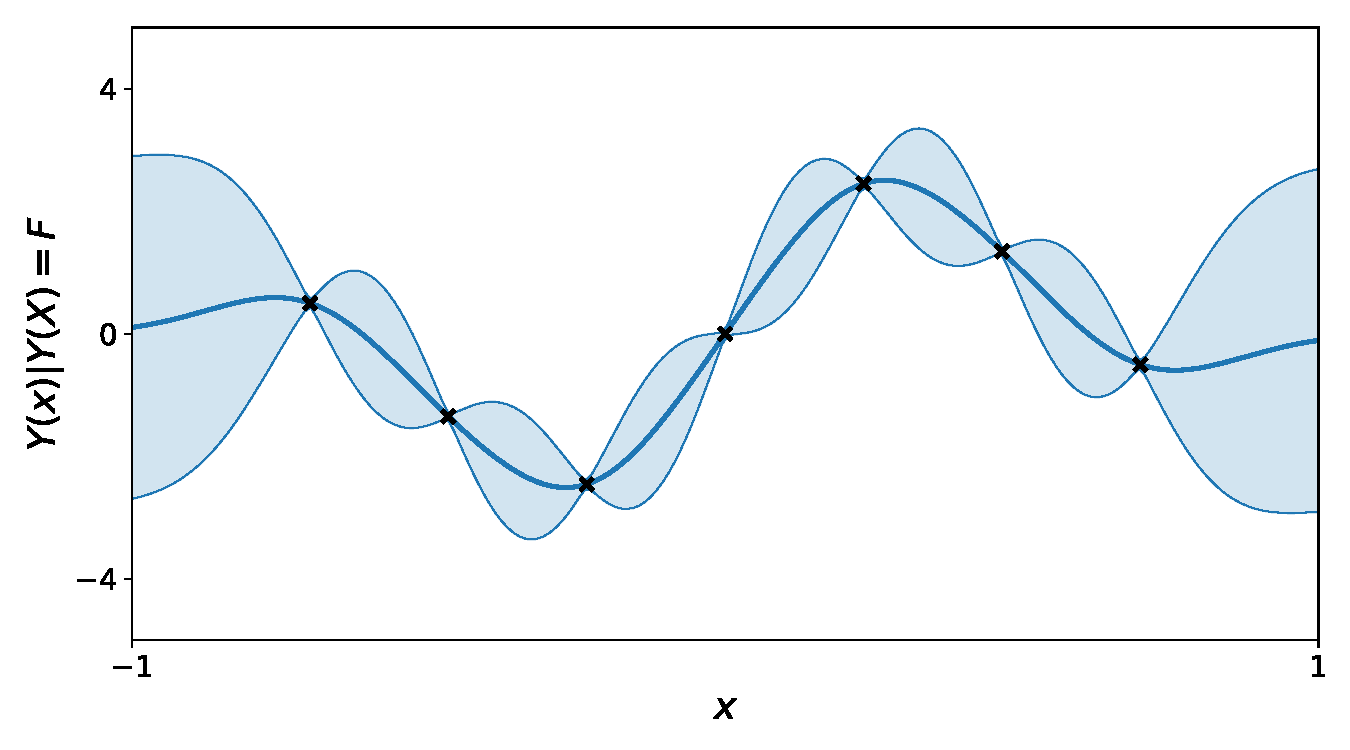
\includegraphics[height=6cm]{figures/python/gp_model}
\end{frame}


%%%%%%%%%%%%%%%%%%%%%%%%%%%%%%%%%%%%%%%%%%%%%%%%%%%%%%
\begin{frame}{}
A few remarkable properties of GPR models
\begin{itemize}
	\item They (can) interpolate the data-points
	\item The prediction variance does not depend on the observations
	\item The mean predictor does not depend on the variance parameter
	\item They (usually) come back to zero when we are far away from the observations.
\end{itemize}
Can we prove them?
\end{frame}


%%%%%%%%%%%%%%%%%%%%%%%%%%%%%%%%%%%%%%%%%%%%%%%%%%%%%%
\begin{frame}{}
Changing the kernel \alert{has a huge impact on the model}:\\
\vspace{5mm}
\begin{center}
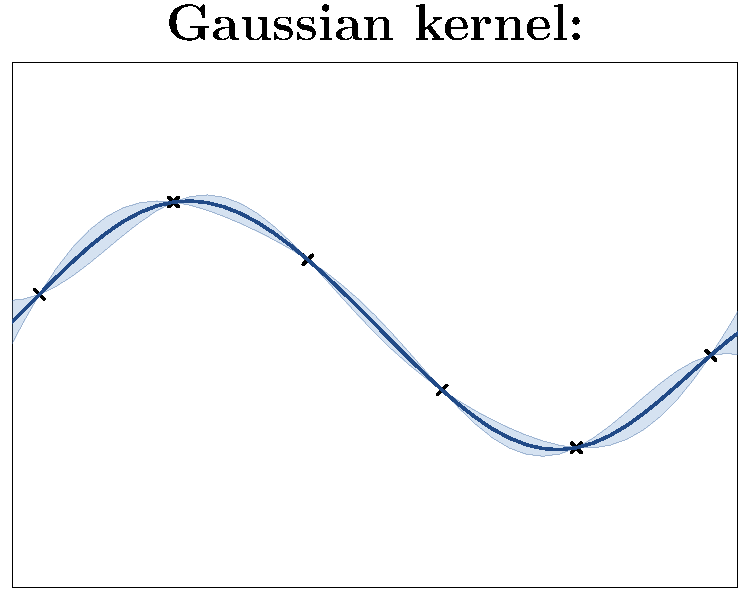
\includegraphics[height=3.9cm]{figures/Fig2-GP-rbf} \qquad
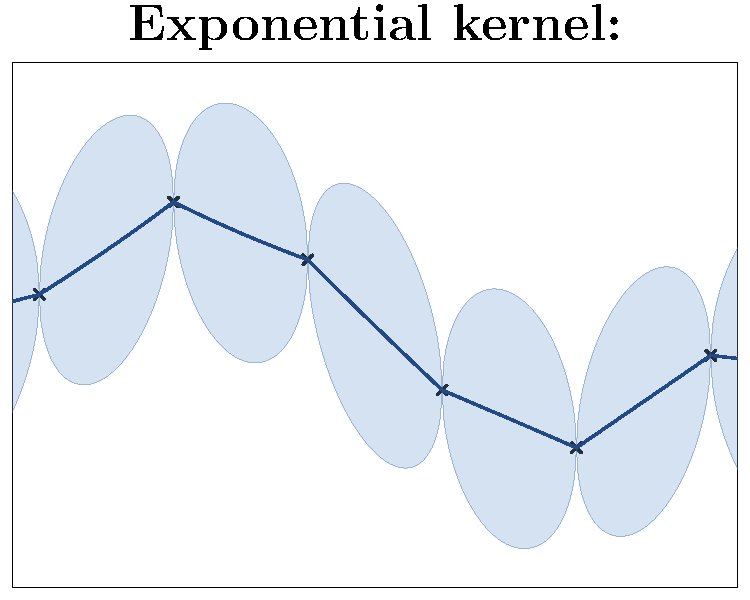
\includegraphics[height=3.9cm]{figures/Fig2-GP-exp}
\end{center}
\end{frame}

%%%%%%%%%%%%%%%%%%%%%%%%%%%%%%%%%%%%%%%%%%%%%%%%%%%%%%
\begin{frame}{}
This is because changing the kernel means changing the prior on $f$\\
\vspace{5mm}
\begin{center}
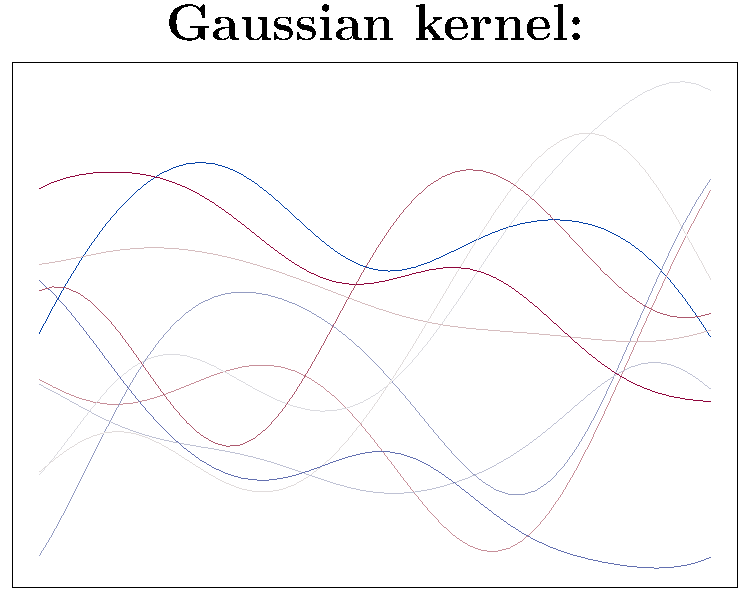
\includegraphics[height=3.8cm]{figures/Fig2-sim-rbf} \qquad
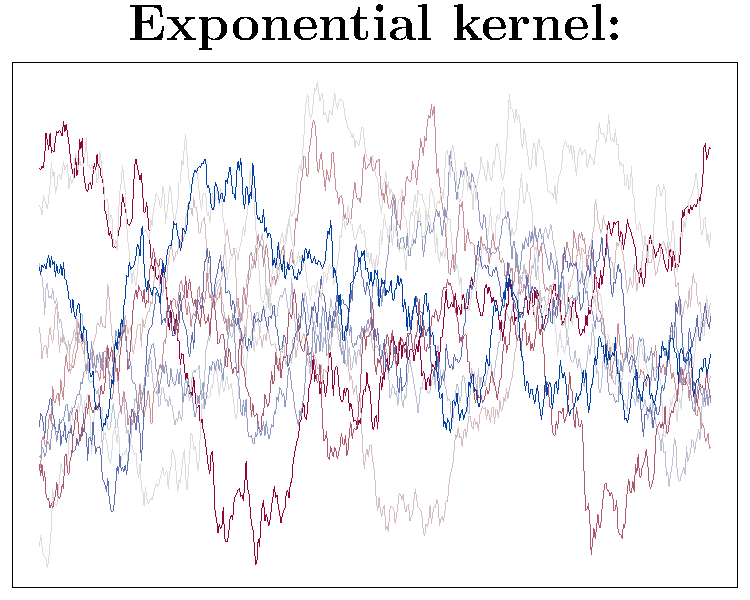
\includegraphics[height=3.8cm]{figures/Fig2-sim-exp}
\end{center}
\end{frame}

%%%%%%%%%%%%%%%%%%%%%%%%%%%%%%%%%%%%%%%%%%%%%%%%%%%%%%
\begin{frame}{}
There is no kernel that is intrinsically better... it depends on data!
\begin{center}
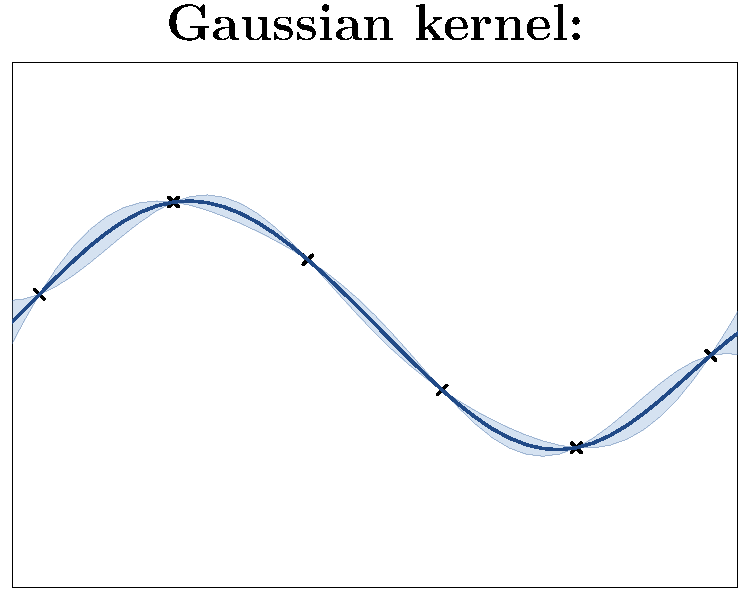
\includegraphics[height=3.5cm]{figures/Fig2-GP-rbf} \hspace{1cm}
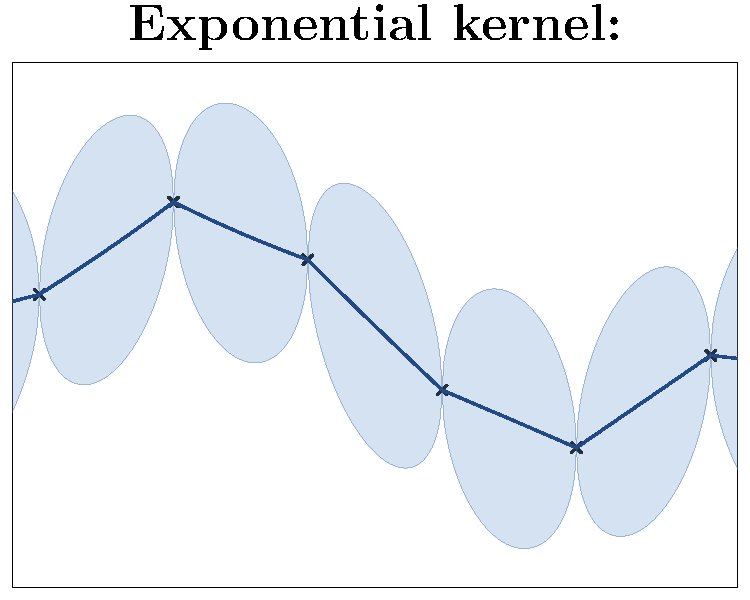
\includegraphics[height=3.5cm]{figures/Fig2-GP-exp}
\end{center}
The kernel has to be chosen accordingly to our prior belief on the behaviour of the function to study:
\begin{itemize}
  \item is it continuous, differentiable, how many times?
  \item is it stationary ?
  \item ...
\end{itemize}
\vspace{5mm}
\alert{$\Rightarrow$ R volcano demo}
\end{frame}

%%%%%%%%%%%%%%%%%%%%%%%%%%%%%%%%%%%%%%%%%%%%%%%%%%%%%%
\begin{frame}{}
We are not always interested in models that interpolate the data. For example, if there is some observation noise: $F = f(X) + \varepsilon$.
\vspace{5mm}
Let $N$ be a process $\mathcal{N}(0,n(.,.))$ that represent the observation noise. The expressions of GPR with noise are
\begin{equation*}
	\begin{split}
	m(x) &= \E[Z(x)|Z(X) + N(X) \shorteq F] \\
	&= k(x,X) (k(X,X)+n(X,X))^{-1} F \\
	& \\
	c(x,y) &= \Cov[Z(x),Z(y)|Z(X)+ N(X) \shorteq F] \\
	&= k(x,y) - k(x,X) (k(X,X)+n(X,X))^{-1} k(X,y)
\end{split}
\end{equation*}
\end{frame}

%%%%%%%%%%%%%%%%%%%%%%%%%%%%%%%%%%%%%%%%%%%%%%%%%%%%%%
\begin{frame}{}
Examples of models with observation noise for $n(x,y)=\tau^2 \delta_{x,y}$:
\begin{center}
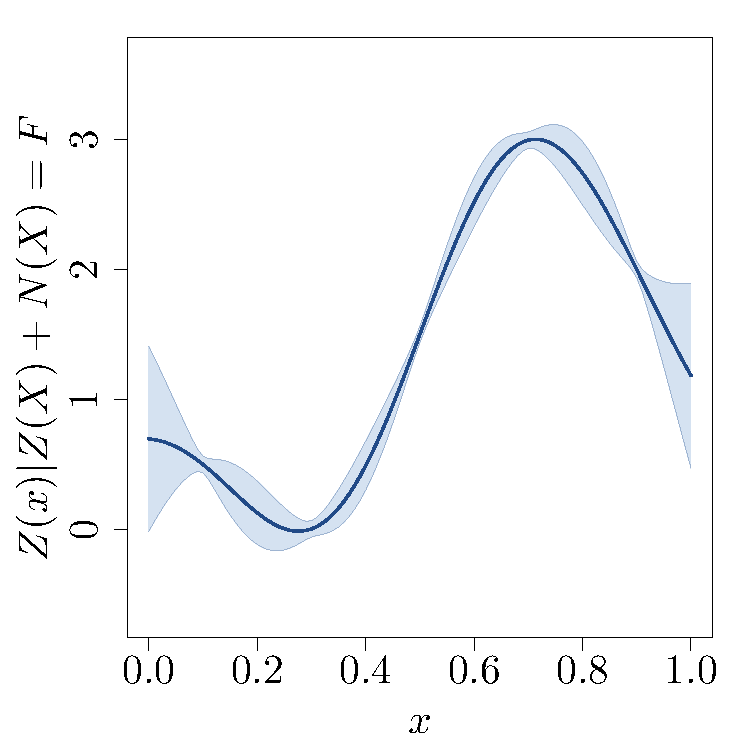
\includegraphics[height=3.5cm]{figures/R/ch34_GPRnoise0001}
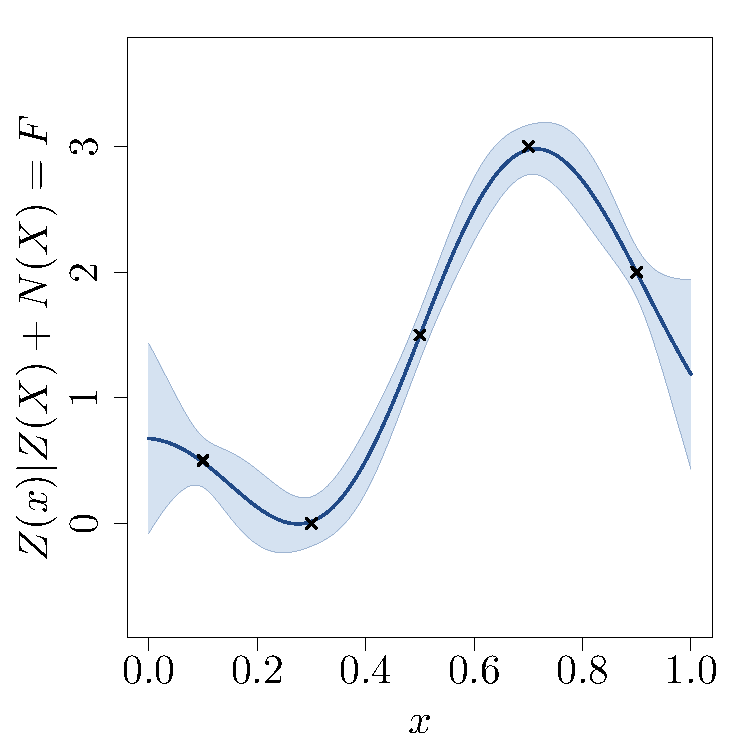
\includegraphics[height=3.5cm]{figures/R/ch34_GPRnoise001}
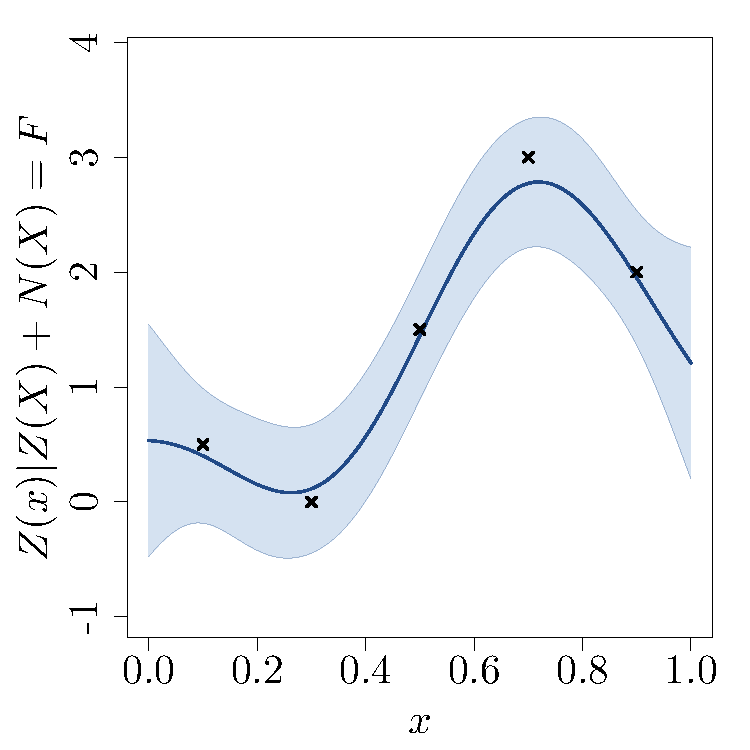
\includegraphics[height=3.5cm]{figures/R/ch34_GPRnoise01}\\
The values of $\tau^2$ are respectively 0.001, 0.01 and 0.1.
\end{center}
\end{frame}

%%%%%%%%%%%%%%%%%%%%%%%%%%%%%%%%%%%%%%%%%%%%%%%%%%%%%%
%%%%%%%%%%%%%%%%%%%%%%%%%%%%%%%%%%%%%%%%%%%%%%%%%%%%%%
\section[Param. estim.]{Parameter estimation}
\subsection{}

%%%%%%%%%%%%%%%%%%%%%%%%%%%%%%%%%%%%%%%%%%%%%%%%%%%%%%
\begin{frame}{}
We have seen previously that the choice of the kernel and its parameters have a great influence on the model. \\ \vspace{5mm}
In order to choose a prior that is suited to the data at hand, we can consider:
\begin{itemize}
	\item minimising the model error
	\item Using maximum likelihood estimation
\end{itemize}
We will now detail the second one.
\end{frame}

%%%%%%%%%%%%%%%%%%%%%%%%%%%%%%%%%%%%%%%%%%%%%%%%%%%%%%
\begin{frame}{}
\begin{definition}
The \textbf{likelihood} of a distribution with a density $f_X$ given some observations $X_1, \dots,X_p$ is:
\begin{equation*}
 	L = \prod_{i=1}^p f_X(X_i)
\end{equation*}
\end{definition}
This quantity can be used to measure the adequacy between observations and a distribution.\\ \vspace{3mm}
\end{frame}

%%%%%%%%%%%%%%%%%%%%%%%%%%%%%%%%%%%%%%%%%%%%%%%%%%%%%%
\begin{frame}{}
In the GPR context, we often have only \textbf{one observation} of the vector $F$. The likelihood is then:
\begin{equation*}
 	L = f_{Z(X)}(F) = \frac{1}{\displaystyle (2 \pi)^{n/2} |k(X,X)|^{1/2}} \exp \left(-\frac12 F^t k(X,X)^{-1} F  \right).
\end{equation*}
It is thus possible to maximise $L$ -- or $\log(L)$ -- with respect to the kernel's parameters in order to find a well suited prior.\\
\vspace{5mm}
\alert{$\Rightarrow$ R demo}
\end{frame}

%%%%%%%%%%%%%%%%%%%%%%%%%%%%%%%%%%%%%%%%%%%%%%%%%%%%%%
%%%%%%%%%%%%%%%%%%%%%%%%%%%%%%%%%%%%%%%%%%%%%%%%%%%%%%
\section{Model validation}
\subsection{}

%%%%%%%%%%%%%%%%%%%%%%%%%%%%%%%%%%%%%%%%%%%%%%%%%%%%%%
\begin{frame}{}
The idea is to introduce new data and to compare the model prediction with reality
\begin{center}
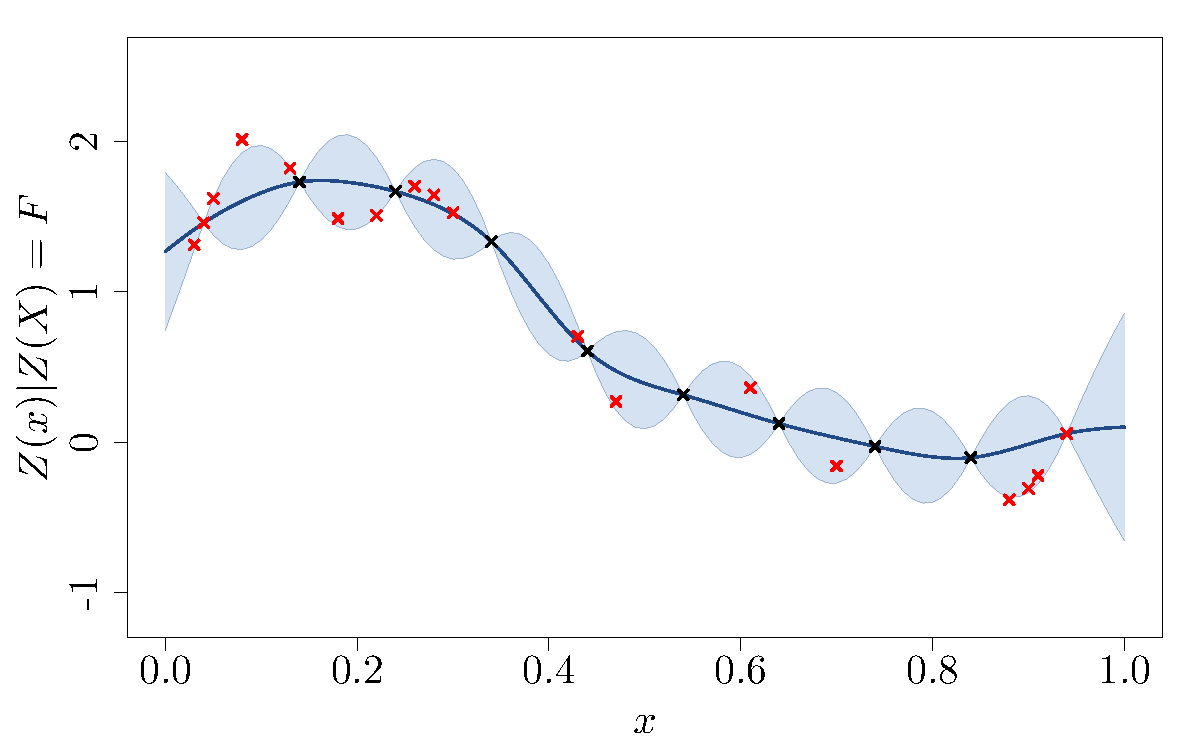
\includegraphics[height=4.5cm]{figures/VALID_testset}
\end{center}
\vspace{3mm}
Since GPR models provide a mean and a covariance structure for the error they both have to be assessed.
\end{frame}

%%%%%%%%%%%%%%%%%%%%%%%%%%%%%%%%%%%%%%%%%%%%%%%%%%%%%%
\begin{frame}{}
Let $X_t$ be the test set and $F_t=f(X_t)$ be the associated observations.\\ \vspace{5mm}
The accuracy of the mean can be measured by computing:
\begin{equation*}
	\begin{split}
		\text{Mean Square Error\qquad}& MSE = \mathrm{mean} ((F_t - m(X_t))^2) \\
		\text{A ``normalised'' criterion\qquad}& Q_2 = 1 - \frac{\sum (F_t - m(X_t))^2}{\sum (F_t - \mathrm{mean}(F_t))^2}
	\end{split}
\end{equation*}
\\ \ \\
On the above example we get $MSE = 0.038$ and $Q_2 = 0.95$.
\end{frame}

%%%%%%%%%%%%%%%%%%%%%%%%%%%%%%%%%%%%%%%%%%%%%%%%%%%%%%
\begin{frame}{}
The predicted distribution can be tested by normalising the residuals. \\ \vspace{3mm}
According to the model, $F_t \sim \mathcal{N}(m(X_t),c(X_t,X_t))$.\\ \vspace{3mm}
$c(X_t,X_t)^{-1/2}(F_t-m(X_t)) $ should thus be independents $\mathcal{N}(0,1)$:
\begin{center}
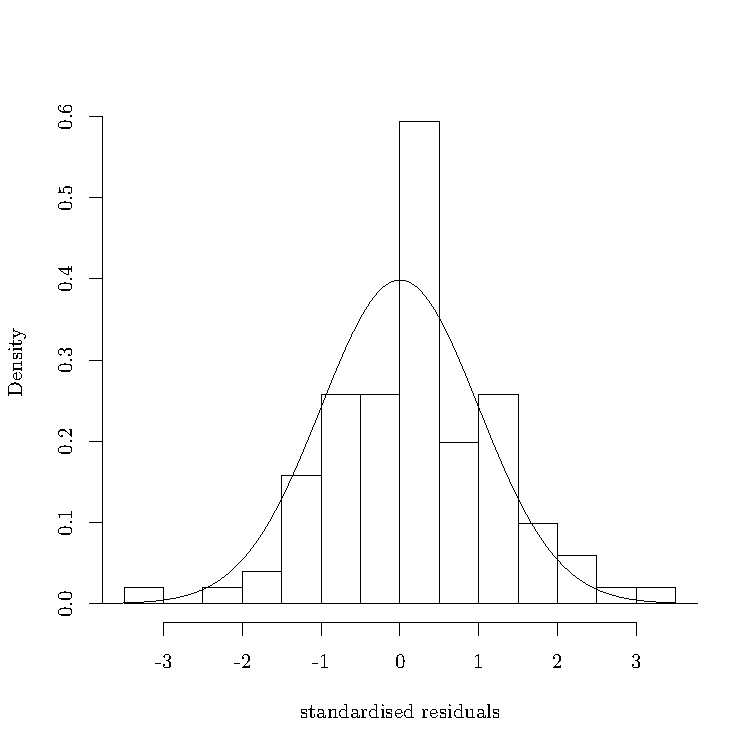
\includegraphics[height=5cm]{figures/VALID_hist} \qquad
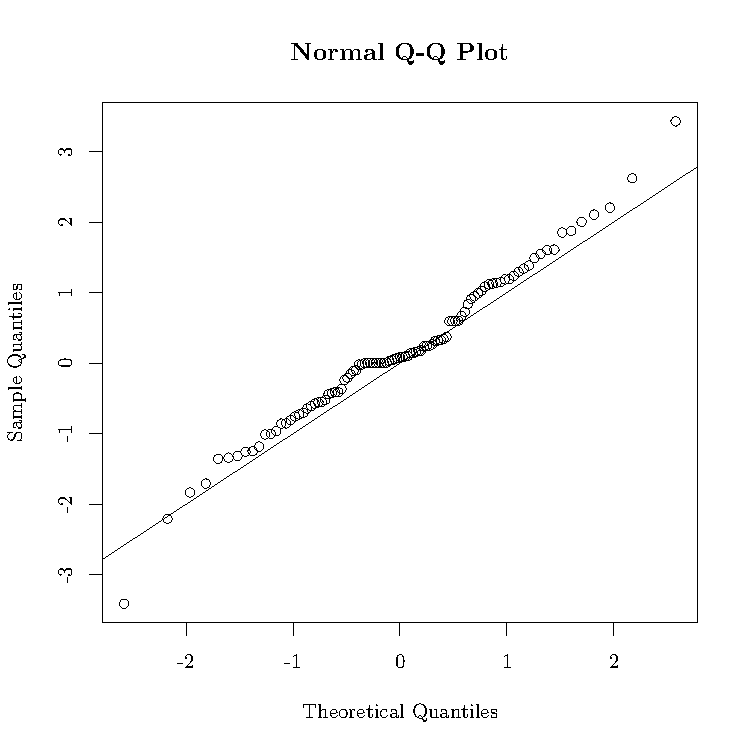
\includegraphics[height=5cm]{figures/VALID_qqplot}
\end{center}
\end{frame}

%%%%%%%%%%%%%%%%%%%%%%%%%%%%%%%%%%%%%%%%%%%%%%%%%%%%%%
\begin{frame}{}
When no test set is available, another option is to consider cross validation methods such as leave-one-out. \\ \vspace{5mm}
The steps are:
\begin{enumerate}
	\item[1.] build a model based on all observations except one
	\item[2.] compute the model error at this point
\end{enumerate}
This procedure can be repeated for all the design points in order to get a vector of error.\\ \vspace{3mm}
\end{frame}

%%%%%%%%%%%%%%%%%%%%%%%%%%%%%%%%%%%%%%%%%%%%%%%%%%%%%%
\begin{frame}{}
Model to be tested:\\ \vspace{3mm}
\begin{center}
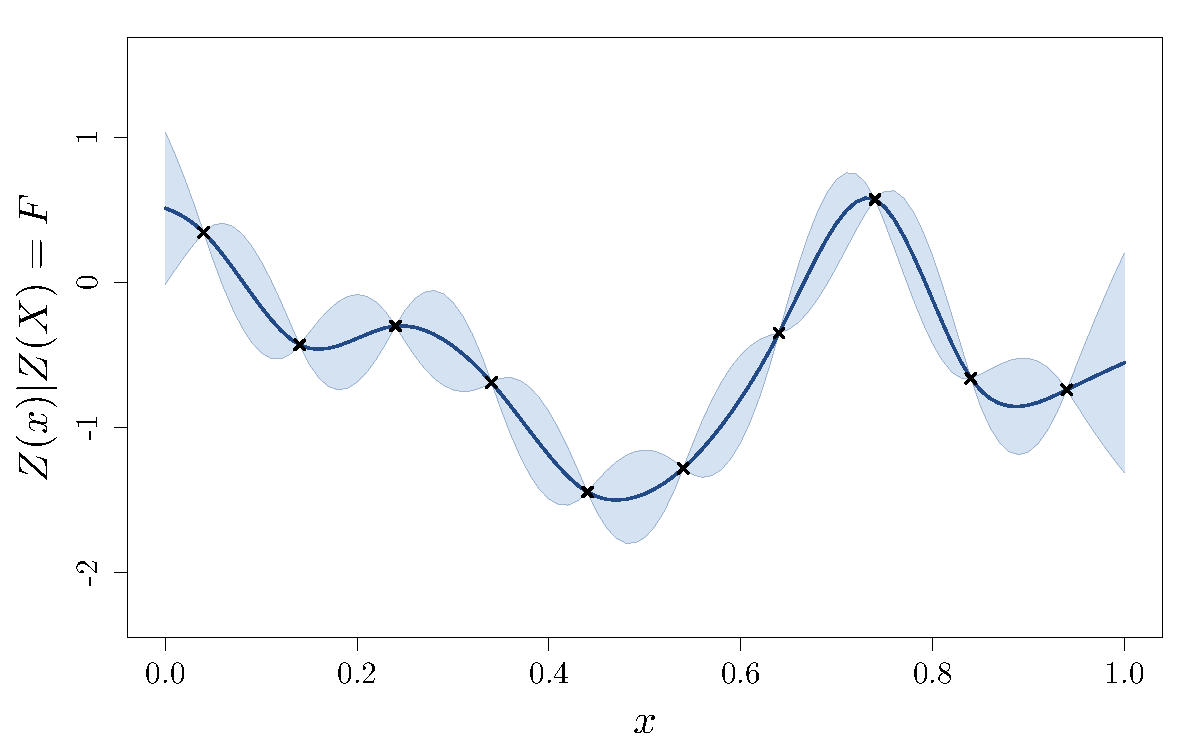
\includegraphics[height=6cm]{figures/VALID_crossval0}
\end{center}
\end{frame}

%%%%%%%%%%%%%%%%%%%%%%%%%%%%%%%%%%%%%%%%%%%%%%%%%%%%%%
\begin{frame}{}
Step 1:\\ \vspace{3mm}
\begin{center}
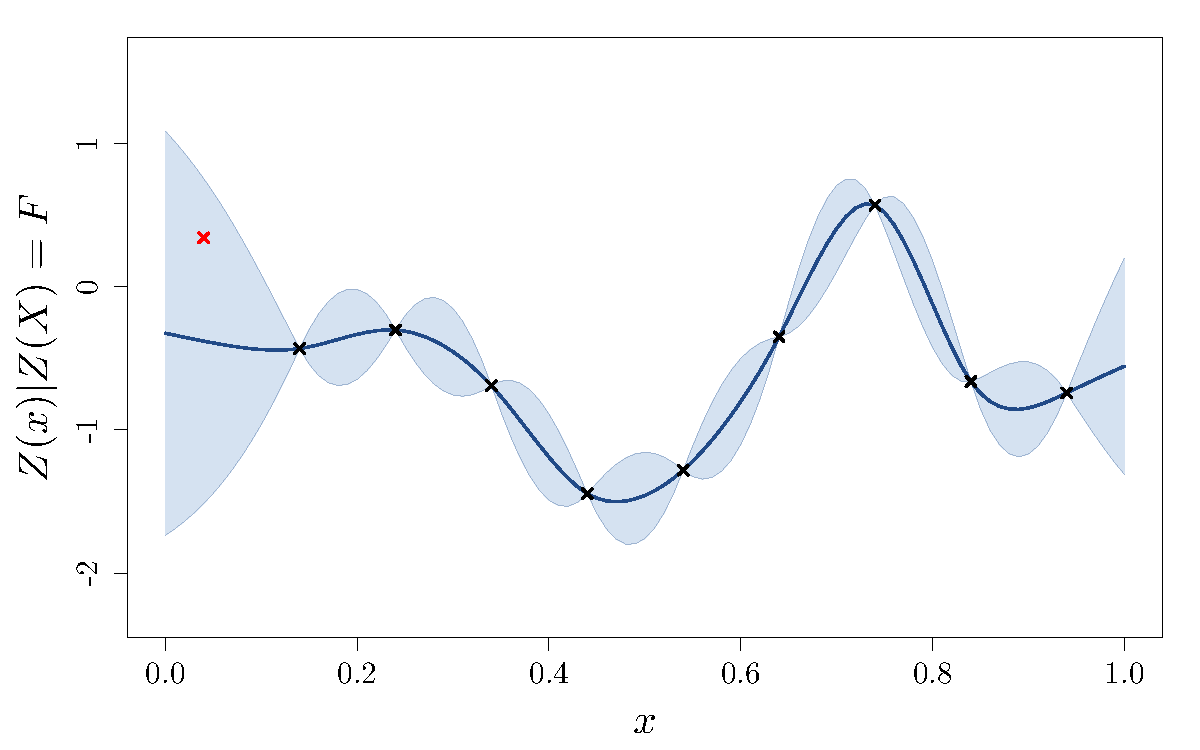
\includegraphics[height=6cm]{figures/VALID_crossval1}
\end{center}
\end{frame}

%%%%%%%%%%%%%%%%%%%%%%%%%%%%%%%%%%%%%%%%%%%%%%%%%%%%%%
\begin{frame}{}
Step 2:\\ \vspace{3mm}
\begin{center}
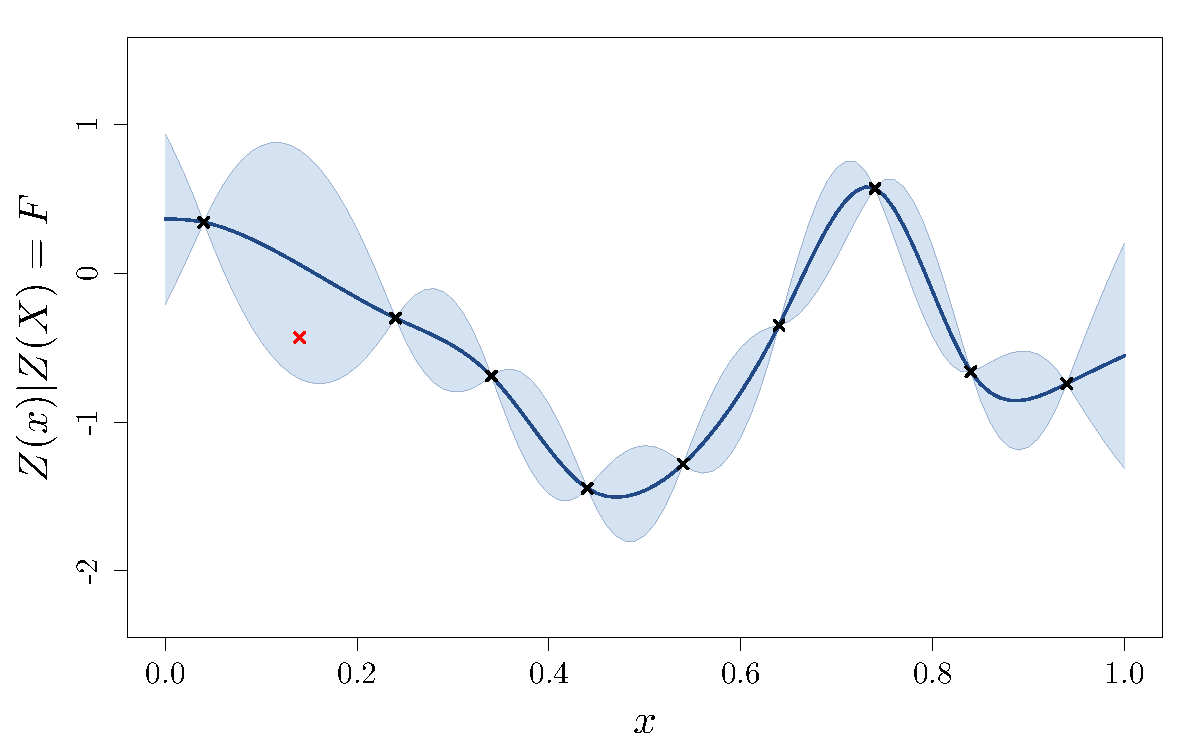
\includegraphics[height=6cm]{figures/VALID_crossval2}
\end{center}
\end{frame}

%%%%%%%%%%%%%%%%%%%%%%%%%%%%%%%%%%%%%%%%%%%%%%%%%%%%%%
\begin{frame}{}
Step 3:\\ \vspace{3mm}
\begin{center}
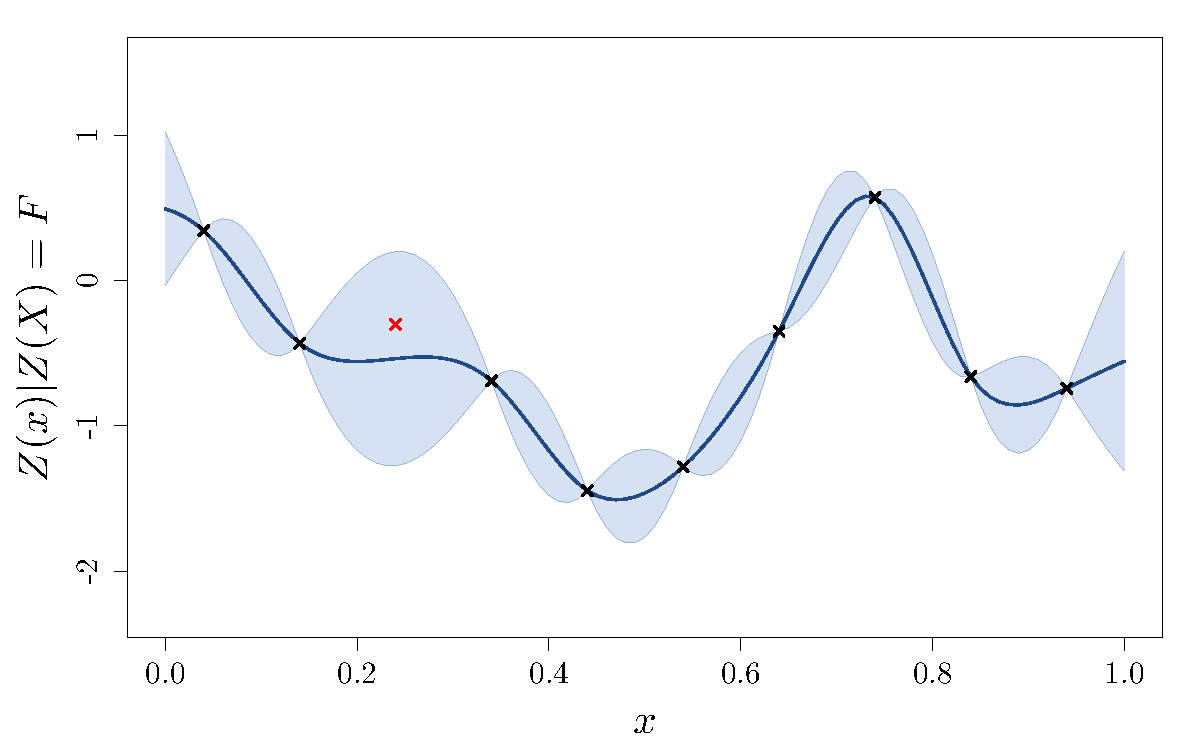
\includegraphics[height=6cm]{figures/VALID_crossval3}
\end{center}
\end{frame}

%%%%%%%%%%%%%%%%%%%%%%%%%%%%%%%%%%%%%%%%%%%%%%%%%%%%%%
\begin{frame}{}
We finally obtain:
 $$MSE = 0.24 \text{ and } Q_2 = 0.34.\vspace{3mm}$$
We can also look at the residual distribution. For leave-one-out, there is no joint distribution for the residuals so they have to be standardised independently.
\begin{center}
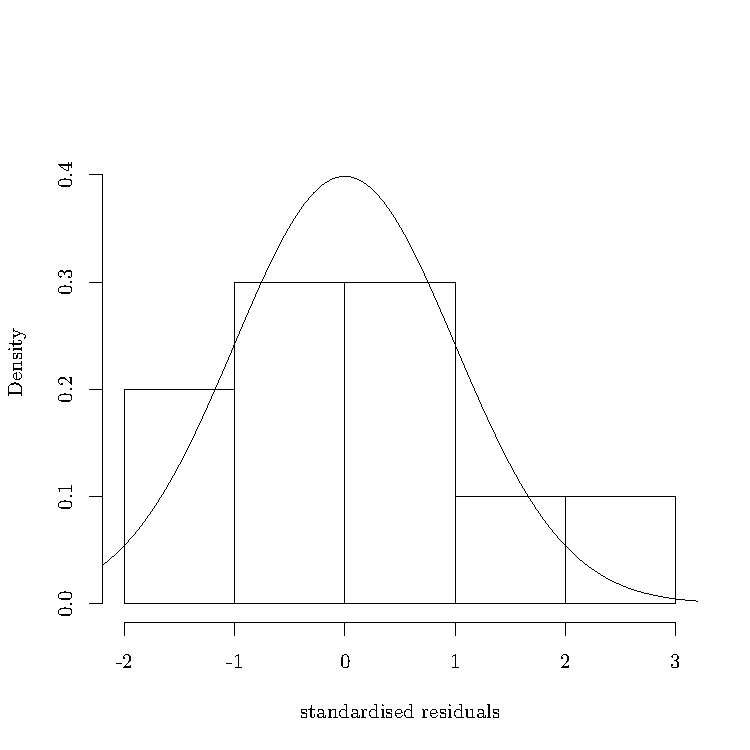
\includegraphics[height=5cm]{figures/VALID_crossvalhist} \qquad
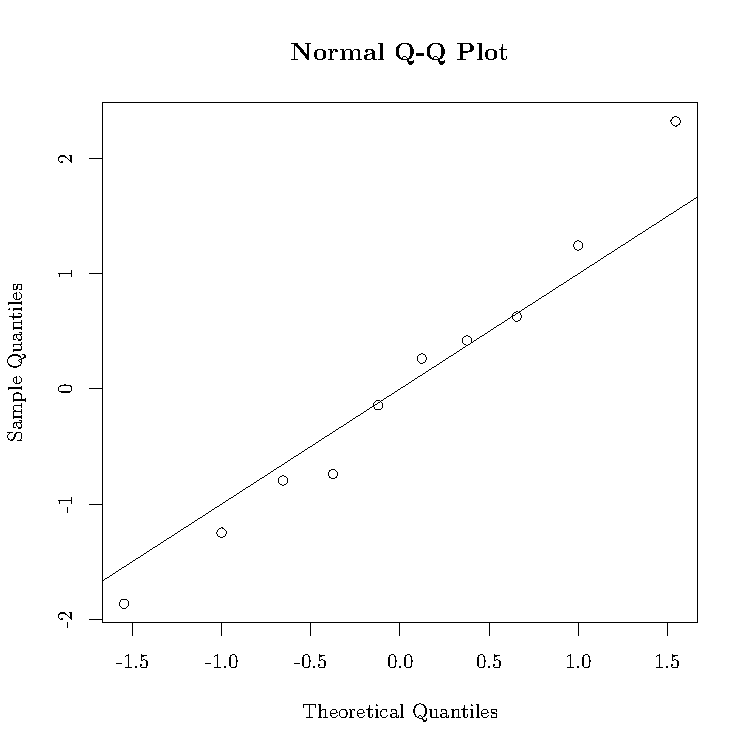
\includegraphics[height=5cm]{figures/VALID_crossvalqqplot}
\end{center}
\end{frame}

%%%%%%%%%%%%%%%%%%%%%%%%%%%%%%%%%%%%%%%%%%%%%%%%%%%%%%
%%%%%%%%%%%%%%%%%%%%%%%%%%%%%%%%%%%%%%%%%%%%%%%%%%%%%%
\section{GPR with trend}
\subsection{}

%%%%%%%%%%%%%%%%%%%%%%%%%%%%%%%%%%%%%%%%%%%%%%%%%%%%%%
\begin{frame}{}
We have seen that GPR models go back to zero if we consider a centred prior. \\ \vspace{5mm} This behaviour is not always wanted
\begin{center}
	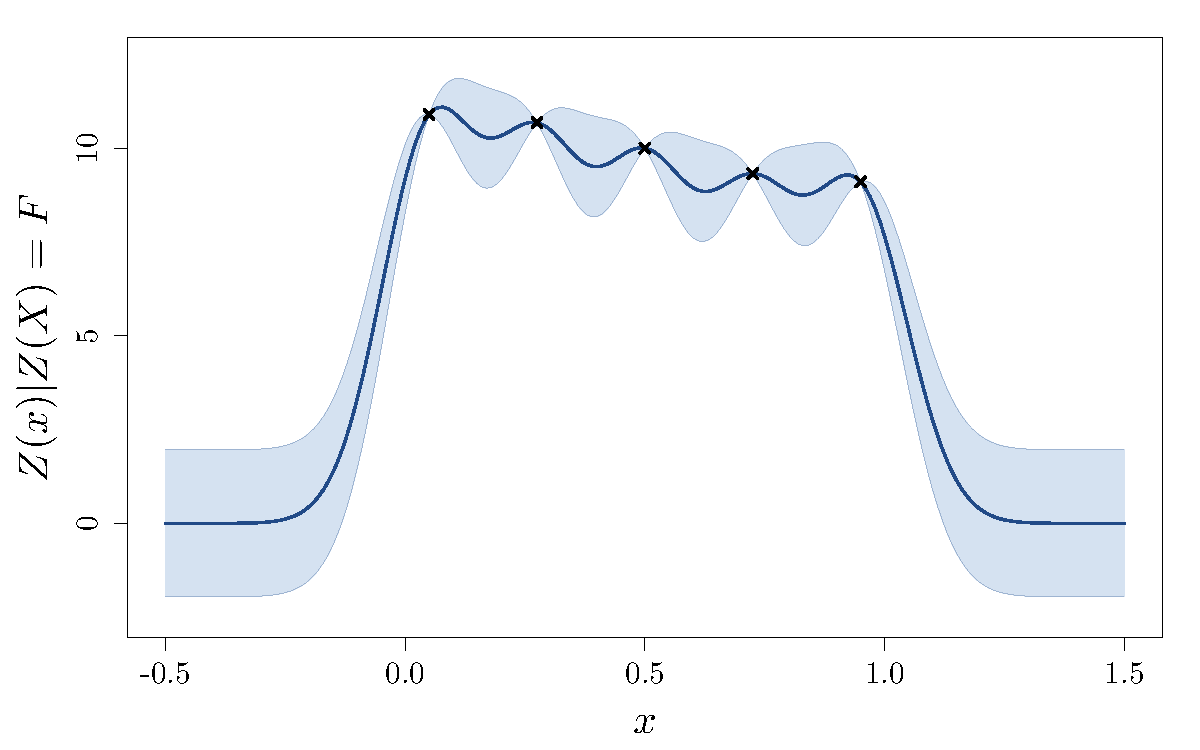
\includegraphics[height=5cm]{figures/R/trend_pb}
\end{center}
\end{frame}

%%%%%%%%%%%%%%%%%%%%%%%%%%%%%%%%%%%%%%%%%%%%%%%%%%%%%%
\begin{frame}{}
If the trend $t(.)$ is known, the usual formulas for multivariate normal conditional distribution apply:
\begin{equation*}
	\begin{split}
		m(x) &= \E[Z(x)|Z(X) \shorteq F] \\
		&= t(x) + k(x,X) k(X,X)^{-1} (F-t(X)) \\ \vspace{3mm}
		c(x,y) &= \Cov[Z(x),Z(y)|Z(X) \shorteq F] \\
		&= k(x,y) - k(x,X) k(X,X)^{-1} k(X,y)
	\end{split}
\end{equation*}
We can see that the trend is subtracted first and then added in the end.
\end{frame}

%%%%%%%%%%%%%%%%%%%%%%%%%%%%%%%%%%%%%%%%%%%%%%%%%%%%%%
\begin{frame}{}
In the previous example, we can consider that trend is constant $t(x)=10$:
\begin{center}
	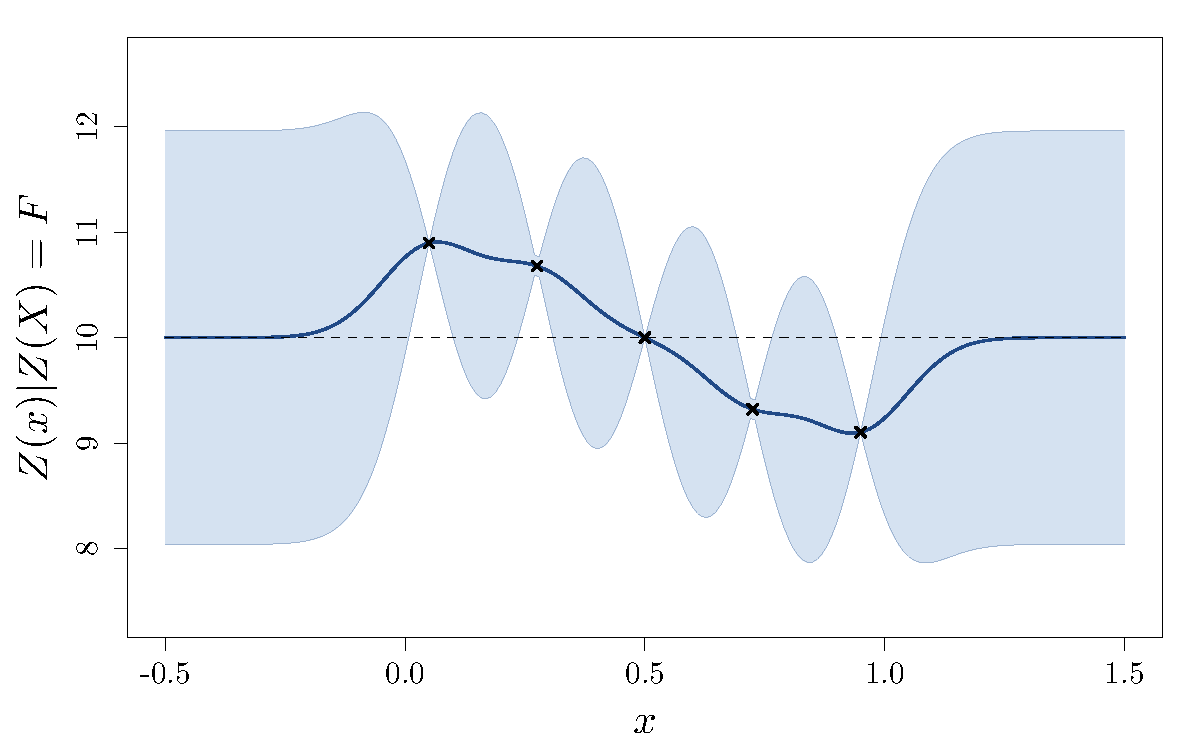
\includegraphics[height=6cm]{figures/R/trend_knowncst}
\end{center}
\end{frame}

%%%%%%%%%%%%%%%%%%%%%%%%%%%%%%%%%%%%%%%%%%%%%%%%%%%%%%
\begin{frame}{}
We can also try a linear trend $t(x)=11-2x$:
\begin{center}
	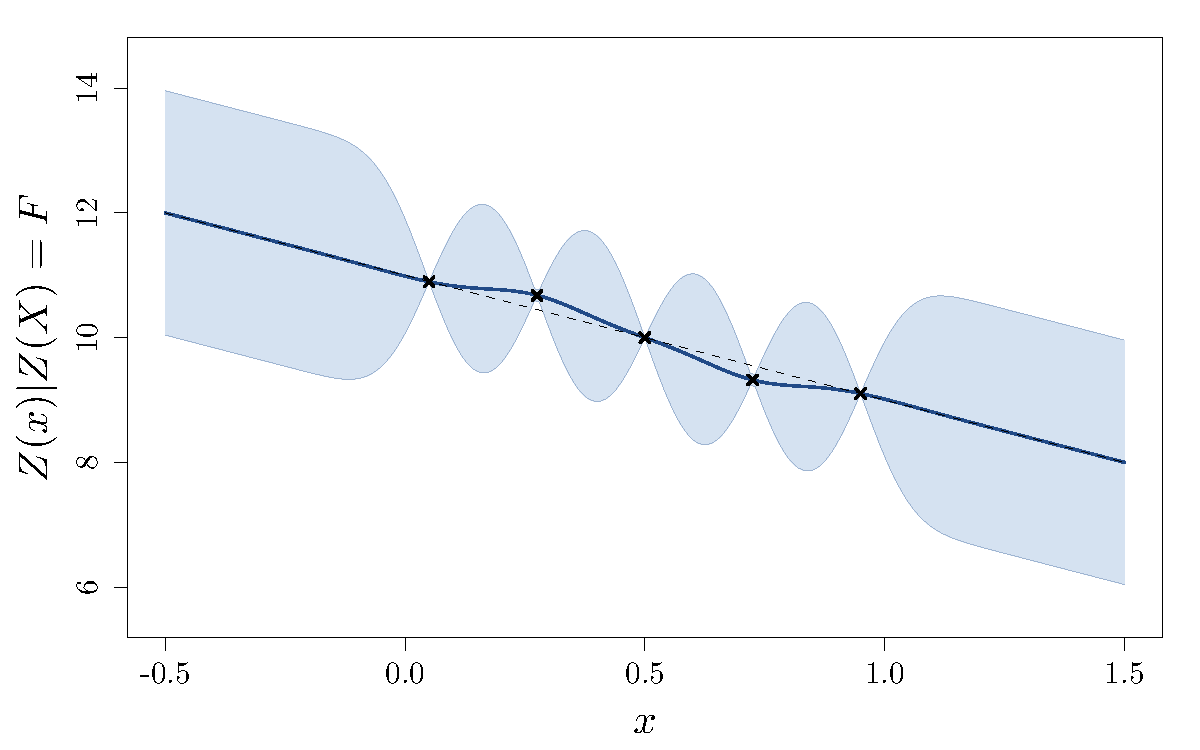
\includegraphics[height=6cm]{figures/R/trend_knownlin}
\end{center}
\end{frame}

%%%%%%%%%%%%%%%%%%%%%%%%%%%%%%%%%%%%%%%%%%%%%%%%%%%%%%
\begin{frame}{}
In practice, the trend is often unknown... The question is then how to estimate it.\\ \vspace{5mm} 
We will distinguish:
\begin{itemize}
	\item \textbf{simple kriging}: there is no trend or it is known
	\item \textbf{ordinary kriging}: the trend is a constant
	\item \textbf{universal kriging}: the trend is given by basis functions
\end{itemize}
\end{frame}

%%%%%%%%%%%%%%%%%%%%%%%%%%%%%%%%%%%%%%%%%%%%%%%%%%%%%%
\begin{frame}{}
    First idea: considering the mean value $t(x) = \text{mean}(F)$... this is not ideal!
\begin{center}
	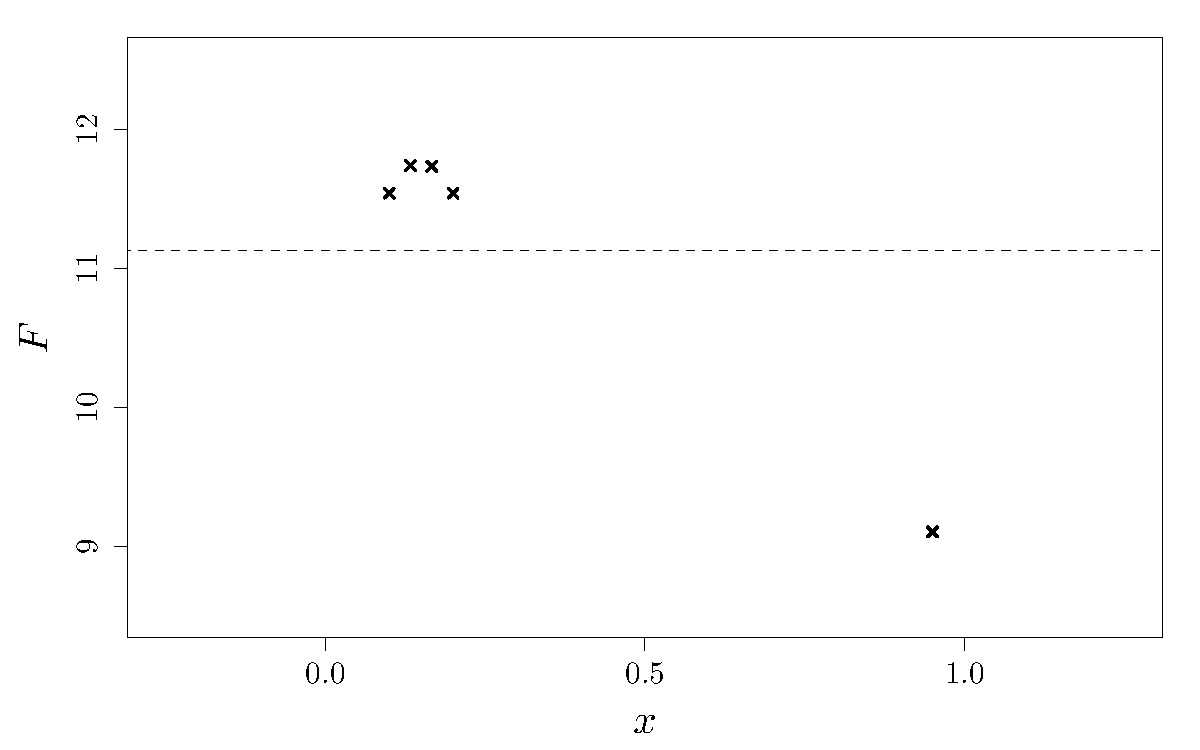
\includegraphics[height=6cm]{figures/R/trend_pbbasicordinary}
\end{center}
Any other idea?
\end{frame}

%%%%%%%%%%%%%%%%%%%%%%%%%%%%%%%%%%%%%%%%%%%%%%%%%%%%%%
\begin{frame}{}
In practice the right thing to to is to find the maximum likelihood value:
\begin{equation*}
L(t) = \frac{1}{\displaystyle (2 \pi)^{n/2} |k(X,X)|^{1/2}} \exp \left(-\frac12 (F-t \mathbf{1})^t k(X,X)^{-1} (F-t \mathbf{1})  \right)
\end{equation*}
\begin{columns}[c]
\begin{column}{4cm}
We obtain:
$$ \hat{t} = \frac{\mathbf{1}^t k(X,X)^{-1} F}{\mathbf{1}^t k(X,X)^{-1} \mathbf{1}}$$ 
\end{column}
\begin{column}{6cm}
\hspace{-8mm} 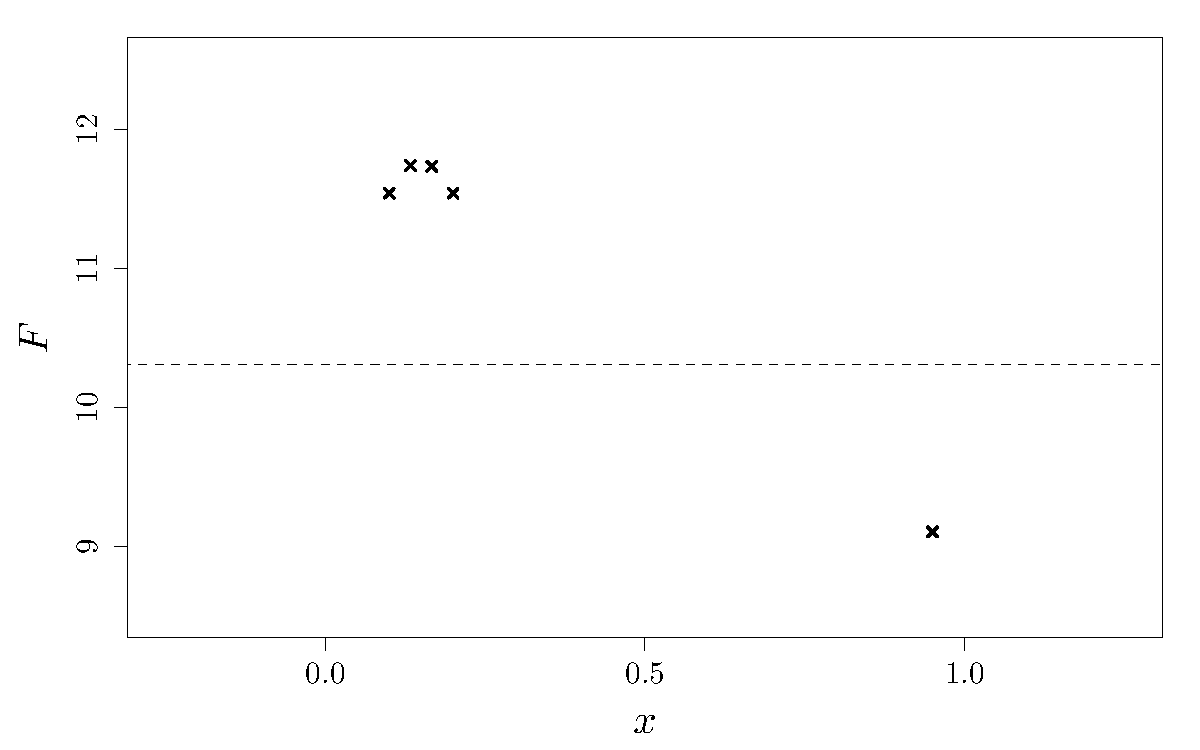
\includegraphics[height=4.2cm]{figures/R/trend_estimordinary}
\end{column}
\end{columns}
\end{frame}

%%%%%%%%%%%%%%%%%%%%%%%%%%%%%%%%%%%%%%%%%%%%%%%%%%%%%%
\begin{frame}{}
The expression of the \textbf{best predictor} is given by the usual conditioning of a GP:
\begin{equation*}
m(x) = \E[Z(x)|Z(X)=F] = \hat{t} - k(x,X) k(X,X)^{-1} (F - \hat{t}) \vspace{5mm}
\end{equation*} 

Regarding the \textbf{model variance}, it must account for the estimator's variance. We will use the law of total Variance :
\begin{equation*}
\Var[X] = \E[\Var(X|Y)] + \Var[\E(X|Y)]
\end{equation*} 
If we apply this to the GPR variance prediction we get:
\small
\begin{equation*}
\begin{split}
\Var[Z(x)|Z(X)] &=  k(x,x) - k(x,X) k(X,X)^{-1} k(X,x)   \\
& \qquad + \frac{(\mathbf{1} + k(x,X)k(X,X)^{-1}\mathbf{1})^t(\mathbf{1} + k(x,X)k(X,X)^{-1}\mathbf{1})}{\mathbf{1}^t k(X,X)^{-1} \mathbf{1}} \\
\end{split}
\end{equation*} 
\normalsize
\end{frame}

%%%%%%%%%%%%%%%%%%%%%%%%%%%%%%%%%%%%%%%%%%%%%%%%%%%%%%
\begin{frame}{}
On the previous example we obtain:
\begin{center}
	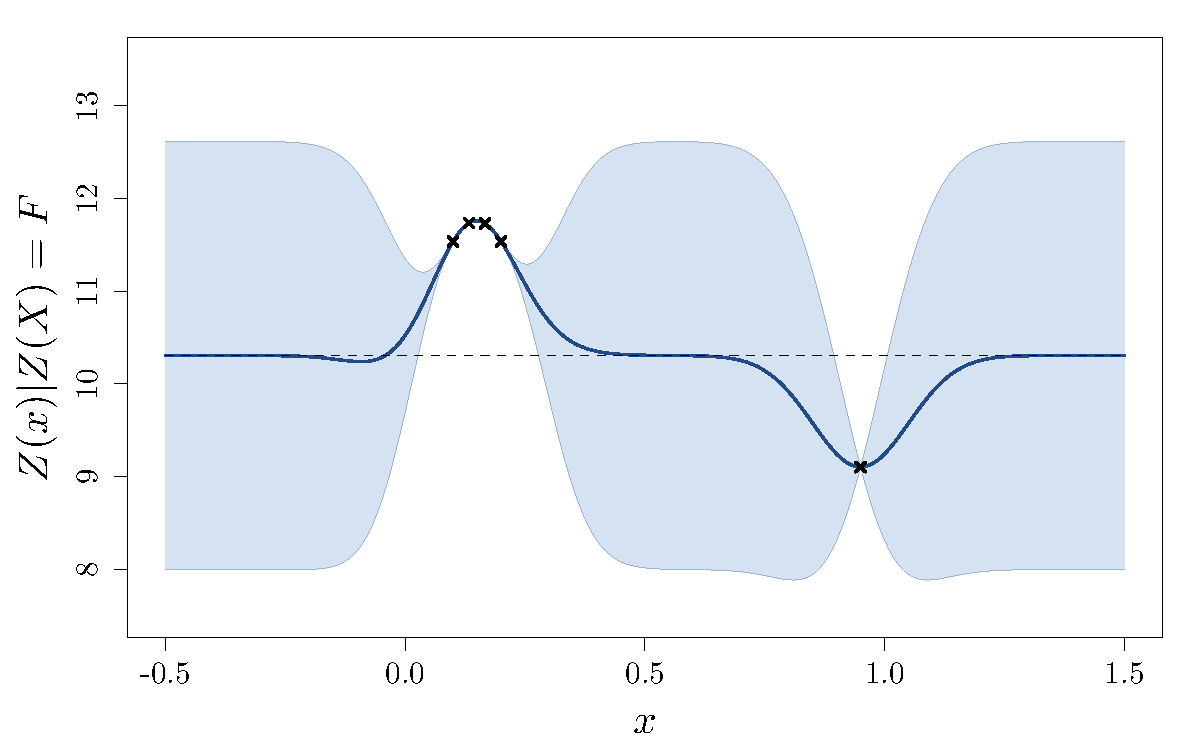
\includegraphics[height=6cm]{figures/R/trend_ko}
\end{center}
\end{frame}

%%%%%%%%%%%%%%%%%%%%%%%%%%%%%%%%%%%%%%%%%%%%%%%%%%%%%%
\begin{frame}{}
it can be compared with simple kriging
\begin{center}
	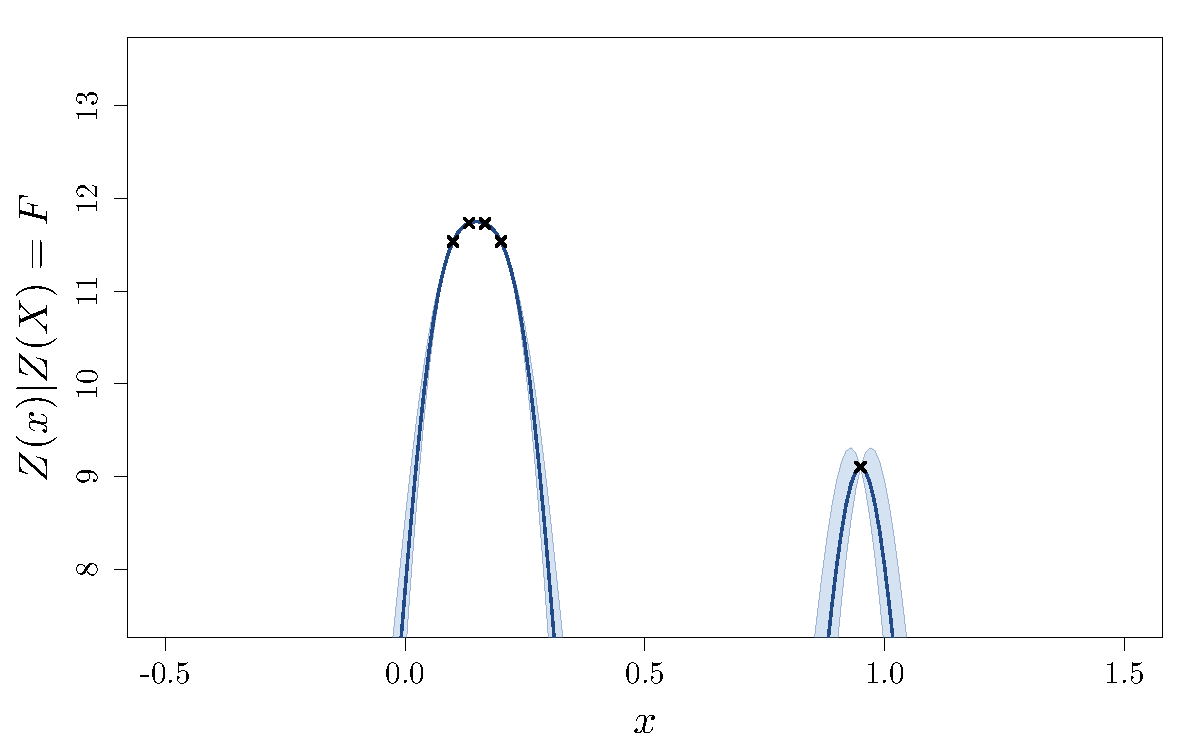
\includegraphics[height=6cm]{figures/R/trend_badks}
\end{center}
\end{frame}

%%%%%%%%%%%%%%%%%%%%%%%%%%%%%%%%%%%%%%%%%%%%%%%%%%%%%%
\begin{frame}{}
If the trend is not constant but linear, quadratic, etc. it is interesting to consider the following probabilistic model for the prior:
\begin{equation*}
	Z(x) = Y(x) + \sum_i \beta_i h_i(x)
\end{equation*}
The model we obtain is called \textbf{universal kriging}. The maximum likelihood estimator gives 
\begin{equation*}
 \hat{\beta} = (H^t k(X,X)^{-1} H)^{-1} H^t k(X,X)^{-1} F 
\end{equation*} 
where $H$ is the matrix of general term $H_{i,j}=h_j(X_i)$.\\
\vspace{5mm}
The final model equations are similar to ordinary kriging. 
\end{frame}

%%%%%%%%%%%%%%%%%%%%%%%%%%%%%%%%%%%%%%%%%%%%%%%%%%%%%%
\begin{frame}{}
We consider the following example
\begin{center}
	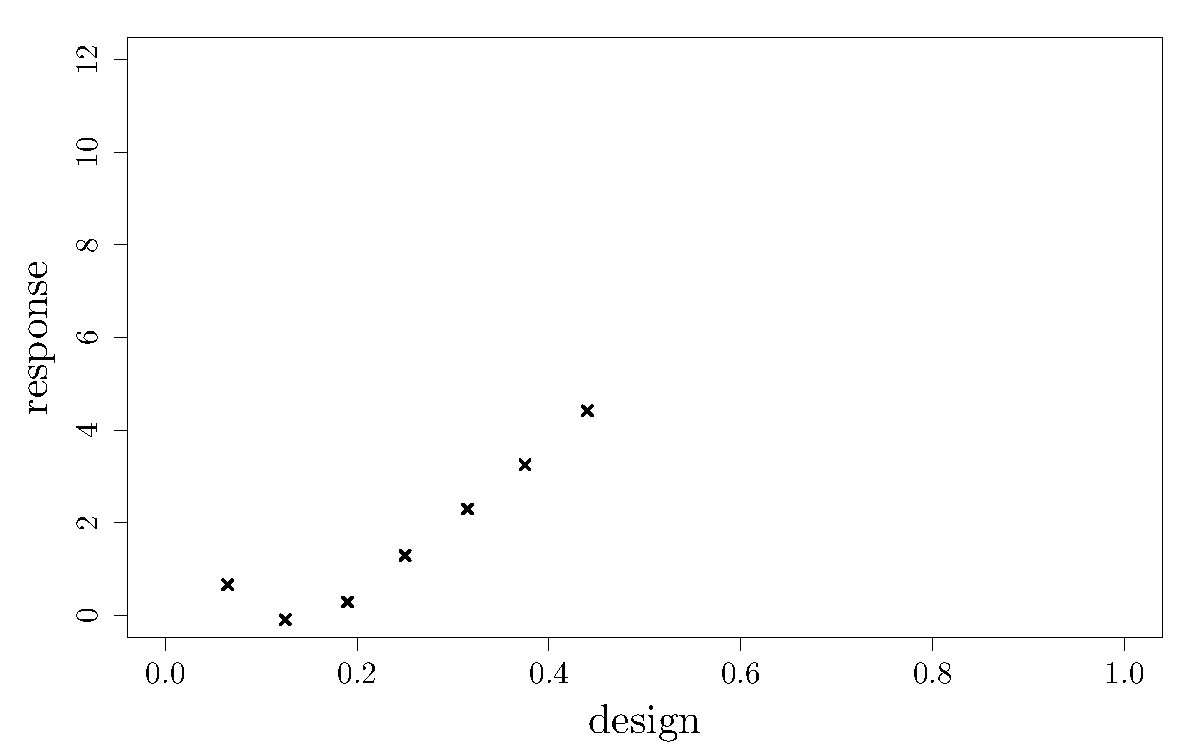
\includegraphics[height=6cm]{figures/R/trend_data}
\end{center}
\end{frame}

%%%%%%%%%%%%%%%%%%%%%%%%%%%%%%%%%%%%%%%%%%%%%%%%%%%%%%
\begin{frame}{}
Universal kriging model with linear trend: $h_1(x) = 1$, $h_2(x) = x$.
\begin{center}
	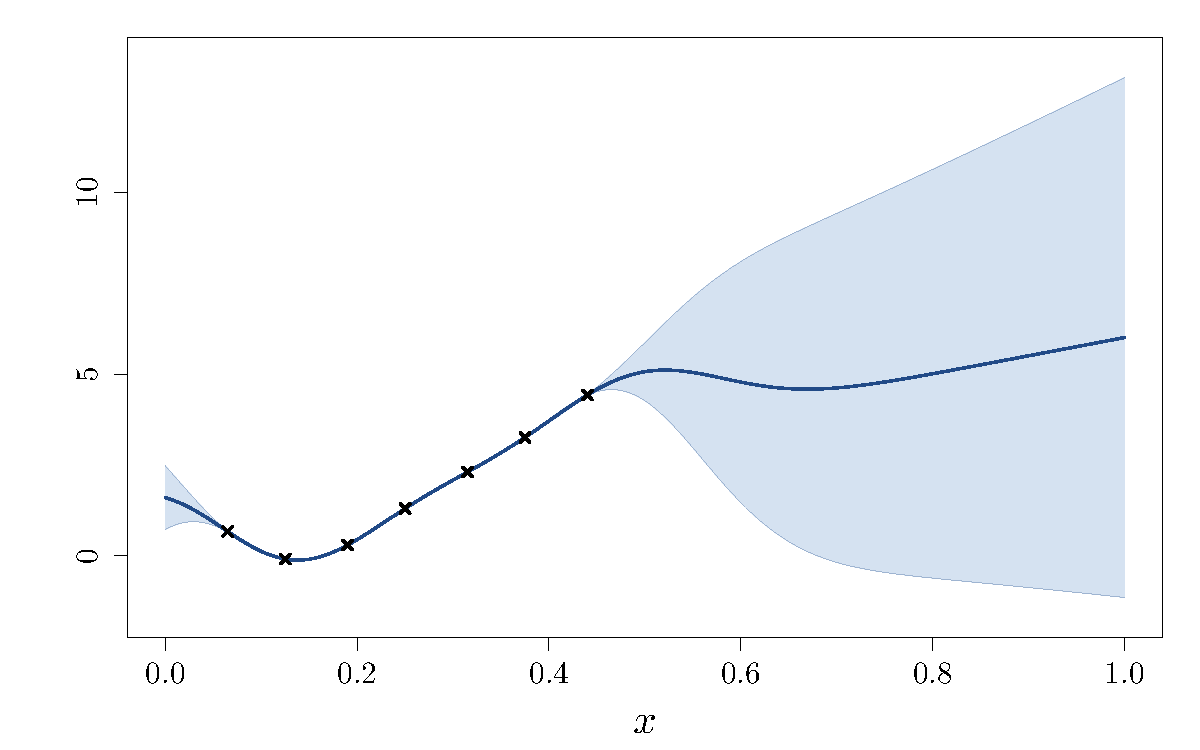
\includegraphics[height=6cm]{figures/R/trend_ku}
\end{center}
\end{frame}

%%%%%%%%%%%%%%%%%%%%%%%%%%%%%%%%%%%%%%%%%%%%%%%%%%%%%%
\begin{frame}{}
It can be compared to simple kriging with known trend
\begin{center}
	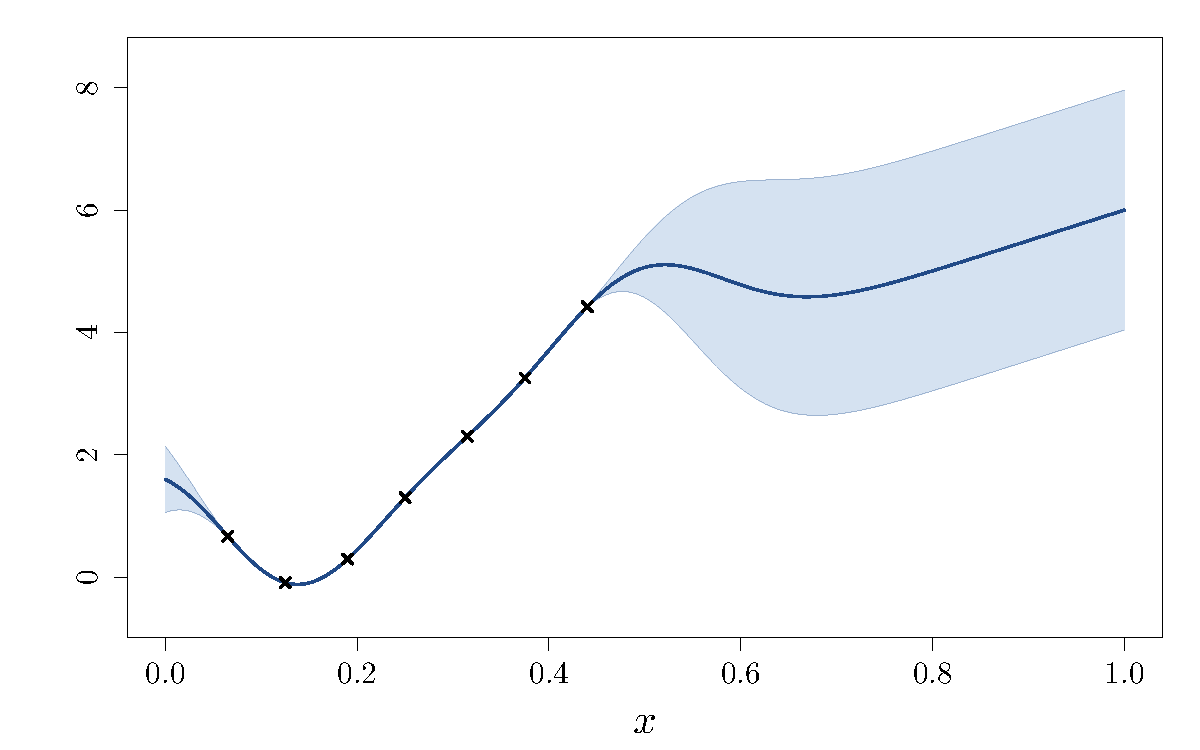
\includegraphics[height=6cm]{figures/R/trend_kstrend}
\end{center}
\end{frame}

%%%%%%%%%%%%%%%%%%%%%%%%%%%%%%%%%%%%%%%%%%%%%%%%%%%%%%%%%%%%%%%%%%%%%%%%
%%%%%%%%%%%%%%%%%%%%%%%%%%%%%%%%%%%%%%%%%%%%%%%%%%%%%%%%%%%%%%%%%%%%%%%%
\section{GPR in practice}
\subsection{}

%%%%%%%%%%%%%%%%%%%%%%%%%%%%%%%%%%%%%%%%%%%%%%%%%%%%%%
\begin{frame}{}
The various steps for building a GPR model are:\\ 
\vspace{3mm}
\begin{enumerate}
	\item Create a DoE
		\begin{itemize}
			\item What is the overall evaluation budget?
			\item What is my model for?
		\end{itemize} \vspace{2mm}
	\item Choose a kernel \vspace{3mm}
	\item Estimate the parameters
		\begin{itemize}
			\item Maximum likelihood
			\item Cross-validation
			\item Multi-start
		\end{itemize} \vspace{2mm}
	\item Validate the model 
		\begin{itemize}
			\item Test set 
			\item Leave-one-out to check mean and confidence intervals
			\item Leave-$k$-out to check predicted covariances
		\end{itemize}
\end{enumerate}
\begin{exampleblock}{Remarks}
	\begin{itemize}
		\item It is common to iterate over steps 2, 3 and 4.
	\end{itemize}
\end{exampleblock}
\end{frame}


%%%%%%%%%%%%%%%%%%%%%%%%%%%%%%%%%%%%%%%%%%%%%%%%%%%%%%
\begin{frame}{}
In practice, the following errors may appear:\\
\begin{itemize}
	\item[\alert{$\bullet$}] \alert{Error: the matrix is not invertible}
	\item[\alert{$\bullet$}] \alert{Error: the matrix is not positive definite}
\end{itemize}
In practice, invertibility issues may arise if observations points are close-by. \\
\vspace{3mm}
This is specially true if
\begin{itemize}
	\item the kernel corresponds to very regular sample paths (squared-exponential for example)
	\item the range (or length-scale) parameters are large
\end{itemize}
\vspace{3mm}
In order to avoid numerical problems during optimization, one can:
\begin{itemize}
	\item add a (very) small observation noise\\
	\item impose a maximum bound to length-scales
	\item impose a minimal bound for noise variance 
	\item avoid the Gaussian kernel
\end{itemize}
\end{frame}

%%%%%%%%%%%%%%%%%%%%%%%%%%%%%%%%%%%%%%%%%%%%%%%%%%%%%%
\begin{frame}{}
A few words on GPR \textbf{Complexity}\\ \vspace{2mm}
	\begin{itemize}
  		\item \structure{Storage footprint:} We have to store the covariance matrix which is $n \times n$.
  		\item \structure{Complexity:} We have to invert the covariance matrix, which requires is $\mathcal{O}(n^3)$.\\
	\end{itemize}
Storage footprint is often the first limit to be reached.\\
\vspace{5mm}
The maximal number of observation points is between $1000$ and $10\,000$.\\
\vspace{2mm}
Note that the complexity do not depend on the dimension of the input space!
\end{frame}


%%%%%%%%%%%%%%%%%%%%%%%%%%%%%%%%%%%%%%%%%%%%%%%%%%%%%%%%%%%%
\section{Conclusion}
\subsection{}

%%%%%%%%%%%%%%%%%%%%%%%%%%%%%%%%%%%%%%%%%%%%%%%%%%%%%%
\begin{frame}{}
\structure{Important points:}\\ \vspace{3mm}
\begin{itemize}
	\item Statistical models are useful when little data is available. they allow to
	\begin{itemize}
		\item interpolate or approximate functions
		\item Compute quantities of interests (such as mean value, optimum, ...)
		\item Get an error measure
	\end{itemize}
	\item GPR is similar to linear regression but the assumption is much weaker (not a finite dimensional space)
\end{itemize}
\vspace{5mm}
\structure{Reference}\\
Carl Edward Rasmussen and Chris Williams, \emph{Gaussian processes for machine learning}, MIT Press, 2006. (free version online).
\end{frame}


%%%%%%%%%%%%%%%%%%%%%%%%%%%%%%%%%%%%%%%%%%%%%%%%%%%%%%%%%%%%%%%%%%%%%%%%%%%%%%%
%%%%%%%%%%%%%%%%%%%%%%%%%%%%%%%%%%%%%%%%%%%%%%%%%%%%%%%%%%%%%%%%%%%%%%%%%%%%%%%
%%%%%%%%%%%%%%%%%%%%%%%%%%%%%%%%%%%%%%%%%%%%%%%%%%%%%%%%%%%%%%%%%%%%%%%%%%%%%%%
%%%%%%%%%%%%%%%%%%%%%%%%%%%%%%%%%%%%%%%%%%%%%%%%%%%%%%%%%%%%%%%%%%%%%%%%%%%%%%%
\end{document}













%%%%%%%%%%%%%%%%%%%%%%%%%%%%%%%%%%%%%%%%%%%%%%%%%%%%%%
%%%%%%%%%%%%%%%%%%%%%%%%%%%%%%%%%%%%%%%%%%%%%%%%%%%%%%
%%%%%%%%%%%%%%%%%%%%%%%%%%%%%%%%%%%%%%%%%%%%%%%%%%%%%%

\structure{}

\begin{center}
  \begin{tabular}{|c|cc|}

  \end{tabular}
\end{center}

###
%%%%%%%%%%%%%%%%%%%%%%%%%%%%%%%%%%%%%%%%%%%%%%%%%%%%%%
\begin{frame}{}

\end{frame}

###
\begin{block}{}

\end{block}

###
\begin{center}
\includegraphics[height=5cm]{figures/}
\end{center}

###
\begin{columns}[c]
\column{5cm}

\column{5cm}

\end{columns}
